\chapter{Implementacja}

Niniejszy rozdział zawiera szczegółową analizę implementacji systemu. Obejmuje on konfigurację komponentów, integrację mechanizmów wykrywania usług i zarządzania zasobami oraz konfigurację narzędzi do monitorowania. Analizując te aspekty implementacji, rozdział ujawnia, w jaki sposób realizowana jest architektura systemu, umożliwiając dynamiczną interakcję między producentami i użytkownikami, efektywną alokację zasobów i solidne monitorowanie wydajności.

\section{Podsystem użytkowy}
\subsection{Rejestr usług}

Głównym elementem w podsystemie użytkowym jest rejestr usług, rejestr ten jest wykorzystywany jako zbiór informacji na temat usług uruchomionych w systemie. W usłudze następuje rejestracja producentów świadczący usługi w systemie oraz węzłów protokołu użytkowników, które są wykorzystywane do zarządzania przydziałem zasobów.

\begin{figure}[!htbp]
    \centering
    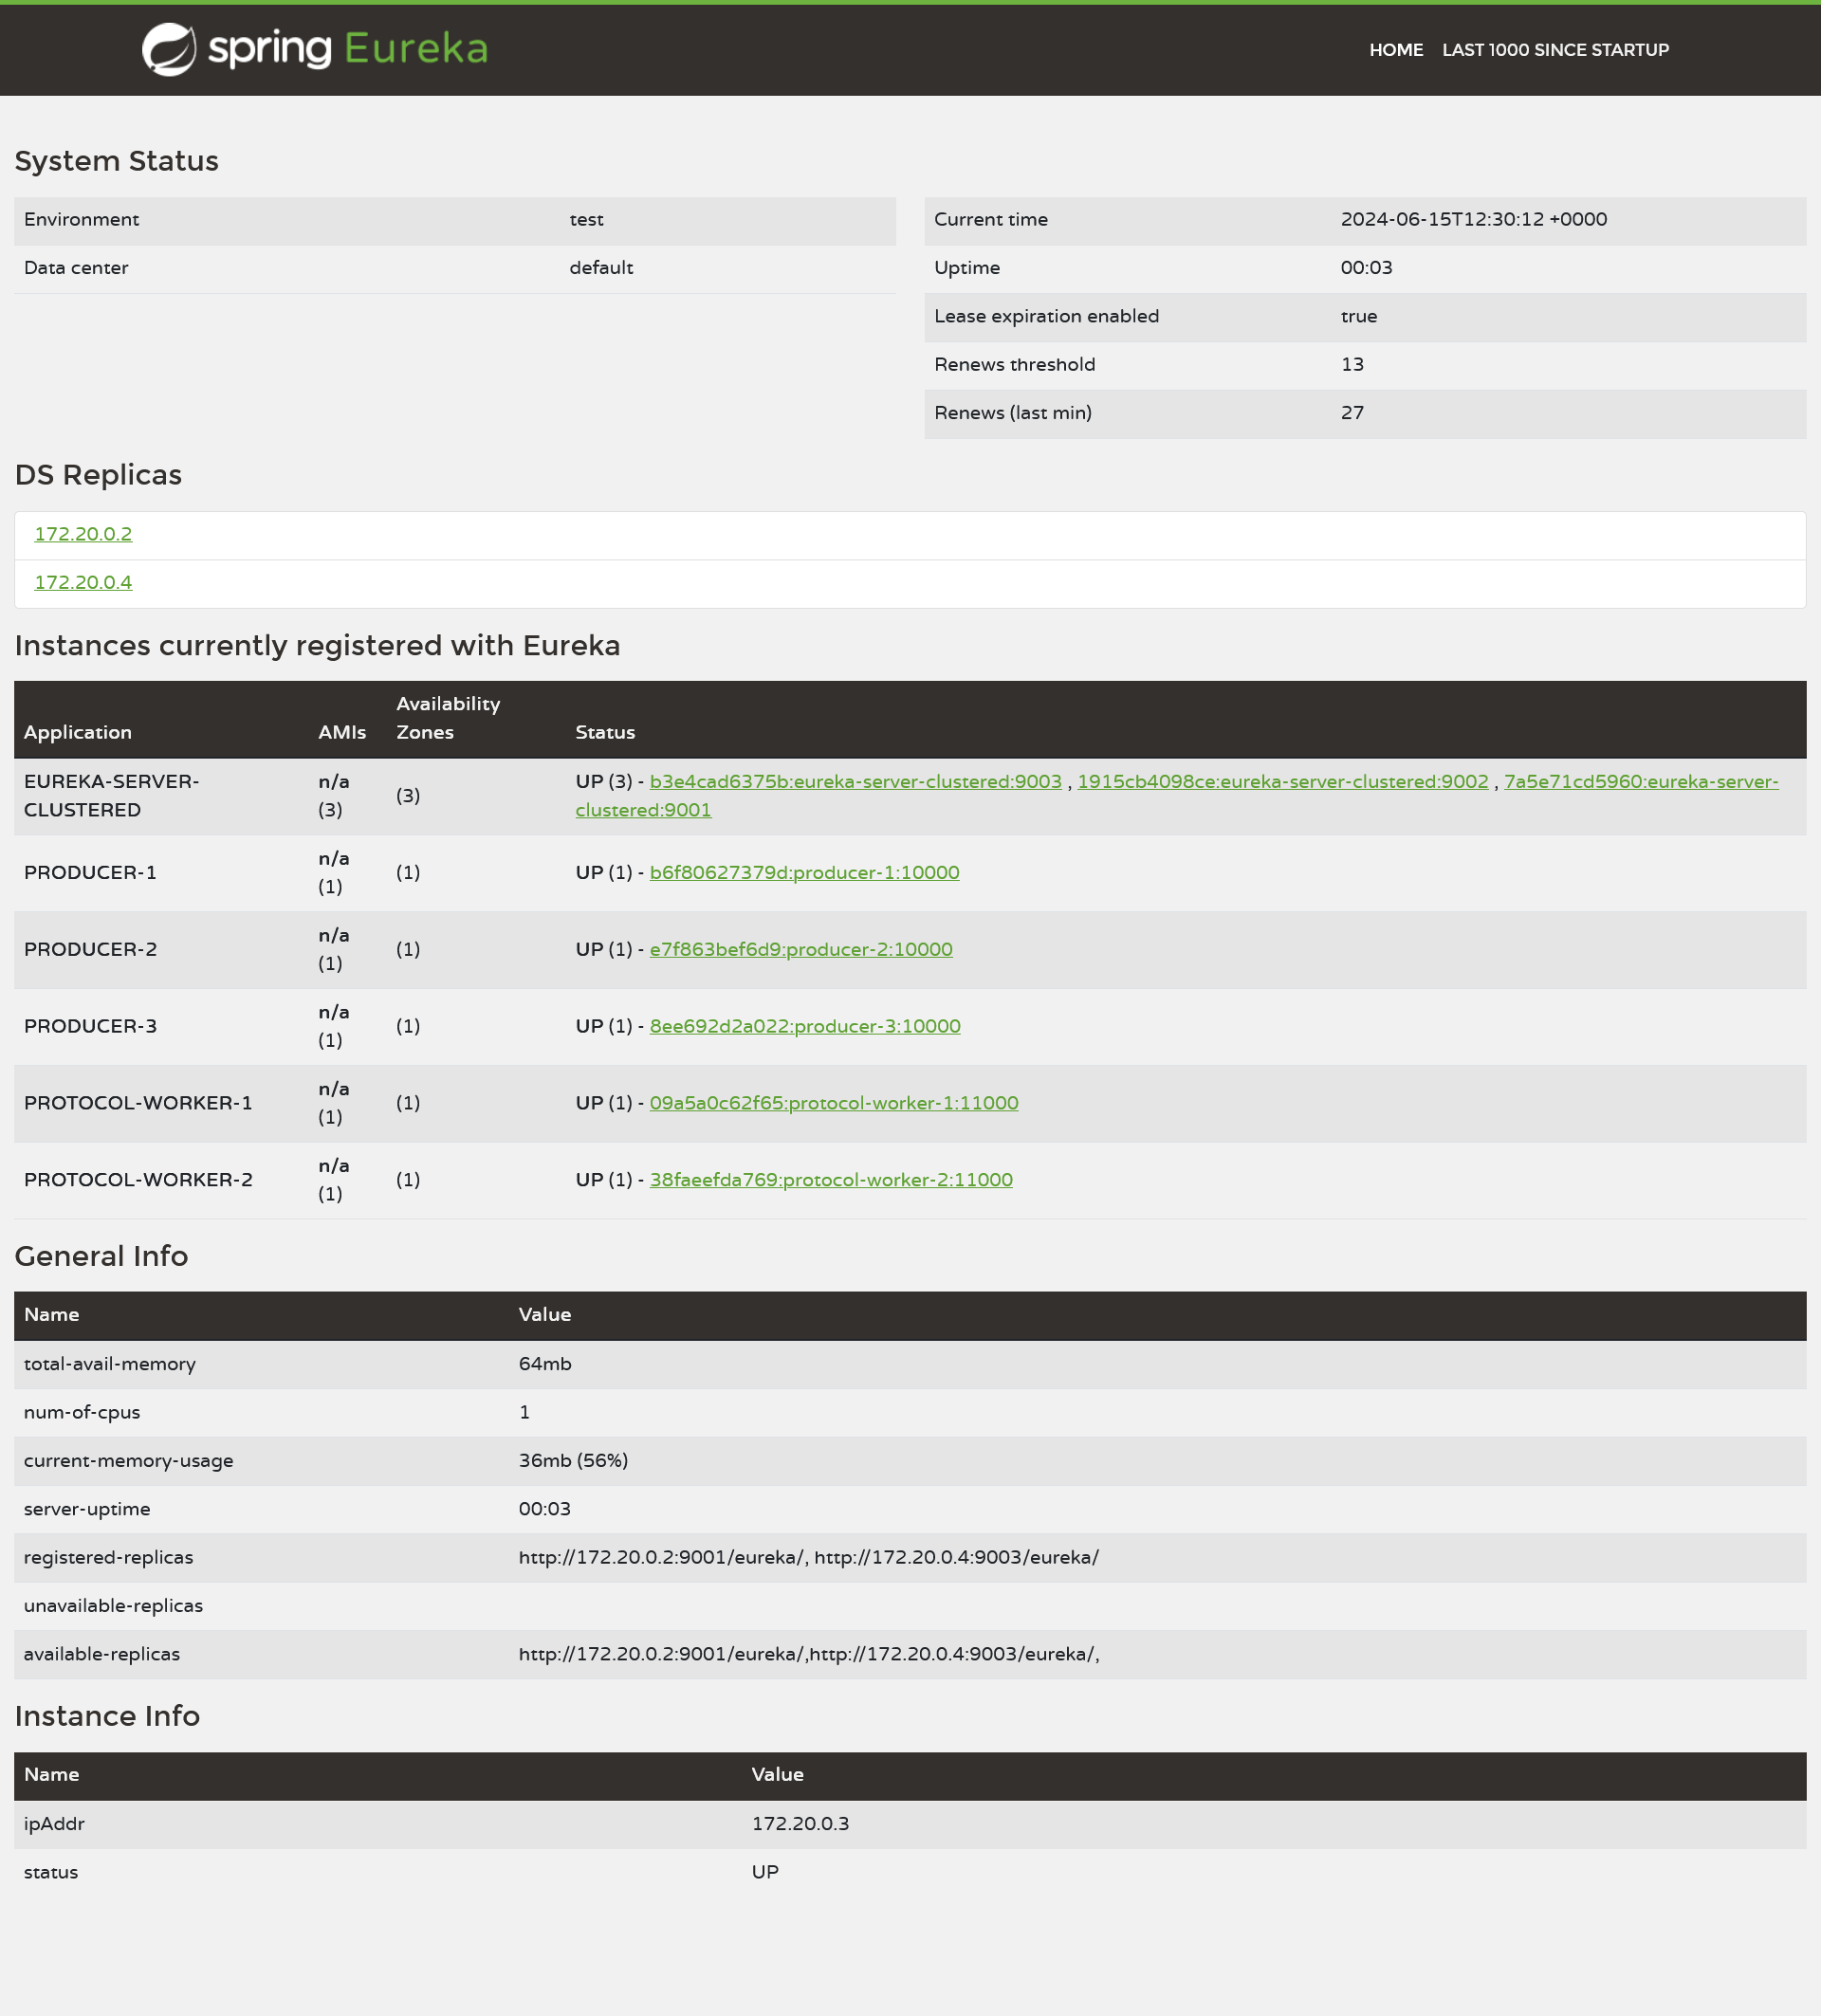
\includegraphics[width=\textwidth]{images/implementation/ServerDiscovery3Producer2Workers.png}
    \caption{Rejestr usług Eureka}
    \label{eurekaServerItems}
\end{figure}

Każda uruchomiona usługa typu producenta oraz węzła protokołu w podsystemie użytkowym jest rejestrowana w usłudze Eureka, gdzie aplikacja przechowywana jest pod unikatową nazwą, która jest wykorzystywana do odpytywania rejestru w usłudze klienckiej w celu otrzymania informacji o działających usługach w systemie. Rejestr przechowuje adresu pod którym usługa jest uruchomiona oraz jej stan. Na rys.\ref{eurekaServerItems} jest przedstawiony przykładowy stan usług zarejestrowanych w rejestrze Eureka.

\begin{lstlisting}[language=Java, caption=Implementacja rejestru usług serwera Eureka]
    
    package com.example.serviceregistry;
    
    import org.springframework.boot.SpringApplication;
    import org.springframework.boot.autoconfigure.SpringBootApplication;
    import org.springframework.cloud.netflix.eureka.server.EnableEurekaServer;
    
    
    @SpringBootApplication
    @EnableEurekaServer
    public class ServiceRegistryApplication {
    
    	public static void main(String[] args) {
    		SpringApplication.run(ServiceRegistryApplication.class, args);
    	}
    }
\end{lstlisting}

Kod usługi rejestru składa się z jednej klasy \verb|ServiceRegistryApplication| oraz metody \verb|main| uruchamiającej aplikacje. Jedyną linijką odróżniającą tę klasę od czystej aplikacji napisanej w frameworku Spring Boot jest adnotacja \verb|@EnableEurekaServer| odpowiada ona za uruchomienie usługi Eureka.

Głównym elementem określającym działanie usługi jest profil Spring Boot oraz wartości przypisane temu profiowi w pliku \verb|application.yml|. 

\subsubsection{Konfiguracja węzła rejestru}

Plik konfiguracyjny \verb|application.yml| jest plikiem YAML podzielony na trzy sekcje, każda opisująca oddzielny profil aplikacji oraz  pola konfiguracyjne niezbędne do prawidłowego działania klastra węzłów rejestru Eureka. 

\begin{lstlisting}[caption=Konfiguracja pierwszego węzła rejestru]
    spring:
      config:
        activate:
          on-profile: peer-1
      application:
        name: eureka-server-clustered
    server:
      port: 9001
    eureka:
      instance:
        preferIpAddress: true
        leaseRenewalIntervalInSeconds: 10
        leaseExpirationDurationInSeconds: 30
      client:
        registerWithEureka: true
        fetchRegistry: true
        serviceUrl:
          defaultZone: ${PEER_2_URL:http://localhost:9002/eureka/},${PEER_3_URL:http://localhost:9003/eureka/}
      server:
        enableSelfPreservation: true
        evictionIntervalTimerInMs: 1000
    logging:
      logstash:
        destinationOne: ${LOGSTASH_DESTINATION_ONE:localhost:5000}
        destinationTwo: ${LOGSTASH_DESTINATION_TWO:localhost:5001}
        destinationThree: ${LOGSTASH_DESTINATION_THREE:localhost:5002}
\end{lstlisting}

\subsubsection{Konfiguracja aplikacji}

Pole \verb|spring.config.activate.on-profile| określa, który profil aplikacyjny będzie aktywny podczas inicjalizacji usługi.

Pole \verb|spring.application.name| ustawia nazwę aplikacji na eureka-server-clustered. Nazwa ta jest wykorzystywana do identyfikacji oraz rejestracji aplikacji w klastrze Eureka.

Pole \verb|server.port| określa port urządzenia na którym aplikacja ma być uruchomiona.

\subsubsection{Konfiguracja instancji Eureka}

Pole \verb|eureka.instance.preferIpAddress| wartość tego pola ustawiona na \verb|true| określa preferowanie przez Eureka adresu \akronim{IP} (\english{Internet Protocol}) zamiast nazwy urządzenia do rejestrowania usług.

Pole \verb|eureka.instance.leaseRenewalIntervalInSeconds| ustawia interwał(w sekundach), co który instancja będzie wysyłać informacje o chęci odnowienia dzierżawy.

Pole \verb|eureka.instance.leaseExpirationDurationInSeconds| określa czas trwania(w sekundach), po którym instancja usługi zostanie uznana za wyłączoną, jeżeli aplikacja nie odnowi dzierżawy.

\subsubsection{Konfiguracja klienta Eureka}

Pole \verb|eureka.client.registerWithEureka| wskazuje, że instancja powinna zarejestrować się w serwerze Eureka.

Pole \verb|eureka.client.fetchRegistry| określa, czy ta instancja powinna pobrać informację z rejestru Eureka.

Pole \verb|eureka.client.serviceUrl.defaultZone| określa adresy \akronim{URL} (\english{Uniform Resource Locator}) usług równorzędnych serwerów Eureka w klastrze.

\subsubsection{Konfiguracja serwera Eureka}

Pole \verb|eureka.server.enableSelfPreservation| określa tryb samozachowawczy, który pomaga w utrzymaniu dostępności serwera Eureka nawet w przypadku partycji sieciowej lub dużych opóźnień.

Pole \verb|eureka.server.evictionIntervalTimerInMs| ustawia interwał (w milisekundach), dla którego ma być uruchamiane zadanie usuwania aplikacji których czas dzierżawy wygasł.

\subsubsection{Konfiguracja logowania zdarzeń}

Pola \verb|logging.logstash.destination*| ustawiają adres do usług zbierających dokumenty, do których będą wysyłane informacje o zdarzeniach w aplikacji producenta. Wykorzystuje zmienną środowiskową LOGSTASH\_DESTINATION\_*, która domyślnie jest ustawiona na localhost:5000, jeśli nie zostanie podana przy uruchomieniu aplikacji.\\[0.5cm]

plik \verb|application.yml| definiuje ustawienia konfiguracyjne dla aplikacji Spring Boot z różnymi profilami: peer-1, peer-2 i peer-3. Każdy profil konfiguruje aplikację jako część klastrowej konfiguracji serwera Eureka oraz wykorzystuje pozostałe uruchomione serwery Eureka jako repliki swojego rejestru w celu zapewnienia wysokiej dostępności w przypadku awarii jednego z węzłów w klastrze.

\subsection{Producent}

Producenci w systemach rozproszonych to komponenty lub usługi odpowiedzialne za generowanie i dostarczanie produktów lub danych. Służą jako źródło informacji lub towarów, które następnie są konsumowane przez inne części systemu. W przedstawianym systemie diagram klas usługi producenta został przedstawiony na rys\ref{ProducerUML}.

\begin{figure}[!htbp]
    \centering
    \includesvg[width=0.65\textwidth]{schemas/producer/Producer.drawio.svg}
    \caption{Producent - schemat UML}
    \label{ProducerUML}
\end{figure}

\subsubsection{Wymagania funkcjonalne}

Usługa producenta powinna spełniać następujące wymagania funkcjonalne:

\begin{itemize}
    \item Producent powinien sprawdzać czy dany produkt znajduje się w jego ofercie.
    \item Producent powinien sprawdzać czy ilość produktów zamawianych przez klienta jest możliwa przez niego do spełnienia. 
    \item Producent powinien zapewnić możliwość odbioru danych w celu sprawdzenia szybkości transmisji między nim a użytkownikiem.
\end{itemize}


\subsubsection{Główna klasa usługi producenta}

Główna klasa usługi producenta przedstawiona na rys\ref{producerMainClass}, jest podstawową klasą uruchamiającą aplikację z wykorzystaniem frameworku Spring Boot. Jest ona oznaczona adnotacją \verb|@EnableDiscoveryClient|, która zapewnia uruchomienie klienta Eureka w celu rejestracji w serwerze Eureka. Adres serwera na, którym aplikacja ma się zarejestrować  ładowany jest z konfiguracji aplikacji.

\begin{lstlisting}[caption=Główna klasa usługi producenta, label=producerMainClass]
    package com.example.producer;

    import org.springframework.boot.SpringApplication;
    import org.springframework.boot.autoconfigure.SpringBootApplication;
    import org.springframework.cloud.client.discovery.EnableDiscoveryClient;
    
    @SpringBootApplication
    @EnableDiscoveryClient
    public class ProducerApplication {
    
        public static void main(String[] args) {
            SpringApplication.run(ProducerApplication.class, args);
        }
    
    }
\end{lstlisting}

\subsubsection{Model produktu}

Klasa \verb|Product| przedstawiona na rys\ref{produktmodel} reprezentuje centralną jednostkę w ramach usługi Producenta.

\begin{lstlisting}[caption=Klasa reprezentująca produkt, label=produktmodel]
    package com.example.producer.model;
    
    import lombok.AllArgsConstructor;
    import lombok.Getter;
    import lombok.NoArgsConstructor;
    import lombok.Setter;
    
    @Getter
    @Setter
    @AllArgsConstructor
    @NoArgsConstructor
    public class Product {
        String id;
        String name;
        String model;
        String producer;
        Integer amount;
        Integer price;
    
        @Override
        public String toString(){
            return "[id = "+
                    id+
                    ", name=" +
                    name +
                    ", model=" +
                    model +
                    ", producer=" +
                    producer +
                    ", amount=" +
                    amount +
                    "price=" +
                    price +
                    "]";
        }
    
    }
\end{lstlisting}

Klasa ta jest opatrzona adnotacjami Lombok, \verb|@Getter|, \verb|@Setter|, które pozwalają automatycznie wygenerować funkcję dostępowe do zmiennych znajdujących się w klasie.

Klasa ta zawiera następujące zmienne:
\begin{itemize}
    \item \verb|String id| - Unikatowe dla danego typu produktu Id
    \item \verb|String name| - Nazwa produktu
    \item \verb|String model| - Model produktu
    \item \verb|String producer| - Nazwa producenta produktu
    \item \verb|Integer amount| - ilość produktu oferowana przez producenta
    \item \verb|Integer price| - cena produktu
\end{itemize}

Klasa ta zawiera metodę \verb|toString()| która przeciąża domyślną metodę klasową języka java \verb|toString()| aby zapewnić reprezentację obiektu produktu, która zawiera wszystkie atrybuty obiektu.

\subsubsection{Serwis Produktów - ProductService}

Klasa \verb|ProductsService| zaprezentowana na listingu\ref{productsServiceCode} jest usługą Spring odpowiedzialną za zarządzanie produktami w aplikacji producenta. Wykorzystuje ona klasę \verb|Product| w celu zainicjowania produktów, przechowywania produktów, oraz pobierania informacji o produktach. Klasa jest opatrzona adnotacją \verb|@Service|, wskazującej że jest to komponent usługi Spring, oraz \verb|@Slf4j|, aby umożliwić tworzenie dziennika zdarzeń w aplikacji.

\begin{lstlisting}[caption=Kod klasy ProductsService, label=productsServiceCode]
    package com.example.producer.service;

    import com.example.producer.model.Product;
    import com.fasterxml.jackson.core.type.TypeReference;
    import com.fasterxml.jackson.databind.ObjectMapper;
    import jakarta.annotation.PostConstruct;
    import lombok.extern.slf4j.Slf4j;
    import org.springframework.beans.factory.annotation.Value;
    import org.springframework.core.io.ClassPathResource;
    import org.springframework.stereotype.Service;
    
    import java.io.IOException;
    import java.io.InputStream;
    import java.util.ArrayList;
    import java.util.Collections;
    import java.util.List;
    import java.util.Optional;
    import java.util.stream.Collectors;
    
    @Service
    @Slf4j
    public class ProductsService {
    
        @Value("${products.file.name}")
        private String productFileName;
    
        @Value("${products.count}")
        private Integer count;
        private List<Product> products = new ArrayList<>();


        @PostConstruct
        public void loadProducts(){
            ObjectMapper objectMapper = new ObjectMapper();
            List<Product> tempProducts;
            try{
                ClassPathResource resource = new ClassPathResource(this.productFileName);
                InputStream in = resource.getInputStream();
                tempProducts = objectMapper.readValue(in, new TypeReference<List<Product>>(){} );
            }catch (IOException e) {
                log.error("Producer was unable to read products from file");
                throw new RuntimeException("Producer was unable to read products from file", e);
            }
            Collections.shuffle(tempProducts);
            this.products = tempProducts.stream().limit(this.count).collect(Collectors.toList());
        }

        public List<Product> getAllProducts() {
            return products;
        }

        public Optional<Product> getProductByName(Product product) {
            return products.stream().filter(listProduct ->  product.getId().equals(listProduct.getId())  && product.getAmount()<= listProduct.getAmount()).findAny();
        }
    }
\end{lstlisting}

Klasa \verb|ProductsService| zawiera następujące zmienne:
\begin{itemize}
    \item \verb|productFileName| - Nazwa pliku przechowującego produktu, z którego są ładowane dane przy starcie aplikacji. Wartość ta jest wstrzykiwana z konfiguracji aplikacji przy użyciu adnotacji \verb|@Value|.
    \item \verb|count| -  Liczba całkowita określająca liczbę produktów do załadowania. Ta wartość jest również wstrzykiwana z konfiguracji aplikacji.
    \item \verb|products| - Lista obiektów \verb|Product| zawierająca załadowane produkty.
\end{itemize}

Klasa \verb|ProductsService| zawiera następujące metody:
\begin{itemize}
    \item \verb|loadProducts| - Metoda opatrzona adnotacją \verb|@PostConstruct| zostaje wywołana automatycznie po inicjalizacji komponentu \verb|ProductsService|. Ładuje ona dane produktów z pliku znajdującego się w głównym folderze aplikacji. Następnie tablica jest mieszana w celu zapewnienia różnych produktów przy każdorazowym uruchomieniu aplikacji. Następnie tablica jest ograniczana do ilości produktów określonej w zmiennej \verb|count|.
    \item \verb|getAllProducts| - metoda zwracająca wszystkie produkty przechowywane w tablicy \verb|products|.
    \item \verb|getProductByName| - Metoda przyjmuje obiekt klasy \verb|Product| jako parametr i zwraca obiekt tej samej klasy opatrzony dodatkową klasą\verb|Optional<>|, który może służyć jako tymczasowy pojemnik z pustą wartość w momencie gdy szukany produkt nie zostanie znaleziony u producenta. W momencie wywołania funkcji tablica jest filtrowana w celu znalezienia czy produkt znajduje się w ofercie producenta oraz czy jego ilość spełnia szukane kryterium przesłane w obiekcie wejściowym.
\end{itemize}

\subsubsection{Kontroler prędkości transmisji - SpeedTestController}

Klasa \verb|speedTestController| przedstawiona na listingu\ref{speedTestControllerCode} zapewnia punkt końcowy do testowania szybkości połączenia pomiędzy producentem a klientem poprzez odbieranie tablicy bajtów i zwracanie bieżącego czasu systemowego w nanosekundach. Punkt końcowy jest mapowany na \verb|/connectionSpeed| i obsługuję żądania \akronim{POST} protokołu \akronim{HTTP} (\english{Hypertext Transfer Protocol}).

\begin{lstlisting}[caption=Kod klasy SpeedTestController, label=speedTestControllerCode]
    package com.example.producer.controllers;

    import lombok.extern.slf4j.Slf4j;
    import org.springframework.http.ResponseEntity;
    import org.springframework.web.bind.annotation.PostMapping;
    import org.springframework.web.bind.annotation.RequestBody;
    import org.springframework.web.bind.annotation.RequestMapping;
    import org.springframework.web.bind.annotation.RestController;
    
    @Slf4j
    @RestController
    @RequestMapping("/connectionSpeed")
    public class SpeedTestController {
    
        @PostMapping
        public ResponseEntity<Long> testSpeed(@RequestBody byte[] data){
            log.info("Received connection speed request, size: {} bytes", data.length);
            return ResponseEntity.ok().body(System.nanoTime());
        }
    }
\end{lstlisting}

\subsubsection{Konfiguracja usługi producenta}

Plik konfiguracyjny przedstawiony na listingu\ref{producerconfigFIle} służy do konfiguracji usługi producenta. Konfiguruje on właściwości aplikacji, ustawienia serwera, konfigurację klienta Eureka, konfigurację dziennika zdarzeń, szczegóły pliku produktów i punkty końcowe zarządzania.

\begin{lstlisting}[caption=Plik konfiguracyjny usługi producenta, label=producerconfigFIle]
    spring:
      application:
        name: producer-${PRODUCER_ID:producer-ERROR}
      servlet:
        multipart:
          max-file-size: 200MB
          max-request-size: 200MB
    
    server:
      port: ${PORT:10000}
      tomcat:
        max-swallow-size: 209715200
        max-http-form-post-size: 209715200
    
    eureka:
      client:
        service-url:
          defaultZone: ${PEER_1_URL:http://localhost:8761/eureka}
        register-with-eureka: true
        fetch-registry: true
    logging:
      logstash:
        destinationOne: ${LOGSTASH_DESTINATION_ONE:localhost:5000}
        destinationTwo: ${LOGSTASH_DESTINATION_TWO:localhost:5001}
        destinationThree: ${LOGSTASH_DESTINATION_THREE:localhost:5002}
    
    #name of products file
    products:
      file:
        name: "products.json"
      count: ${NUMBER_OF_PRODUCTS:1000}
    
    management:
      endpoints:
        web:
          exposure:
            include: "*"
\end{lstlisting}

\subsubsection{Konfiguracja aplikacji}

Pole \verb|spring.application.name| ustawia nazwę aplikacji. Wykorzystuje zmienną środowiskową PRODUCER\_ID, który domyślnie ma wartość "producer-ERROR", jeżeli zmienna środowiskowa nie zostanie podana przy uruchomieniu.

Pole \verb|spring.servlet.multipart.max-file-size| - konfiguruje maksymalny rozmiar pliku dla przesyłania plików wieloczęściowych do 200 MB.

Pole \verb|spring.servlet.multipart.max-request-size| - konfiguruje maksymalny rozmiar żądania dla przesyłania plików wieloczęściowych do 200 MB.

\subsubsection{Konfiguracja serwera aplikacji}

Pole \verb|server.port| ustawia port serwera. Wykorzystuje zmienną środowiskową PORT, która domyślnie wynosi 10000, jeśli nie zostanie podana przy uruchomieniu.

Pole \verb|server.tomcat.max-swallow-size| konfiguruje maksymalny rozmiar odbioru plików dla Tomcat do 200 MB.

Pole \verb|server.tomcat.max-http-form-post-size| konfiguruje maksymalny rozmiar żądania \akronim{POST} formularza \akronim{HTTP} dla serwera Tomcat do 200 MB.

\subsubsection{Konfiguracja logowania zdarzeń}

Pola \verb|logging.logstash.destination*| ustawiają adres do usług zbierających dokumenty, do których będą wysyłane informacje o zdarzeniach w aplikacji producenta. Wykorzystuje zmienną środowiskową LOGSTASH\_DESTINATION\_*, która domyślnie jest ustawiona na localhost:5000, jeśli nie zostanie podana przy uruchomieniu aplikacji.

\subsubsection{Konfiguracja pliku produktów}

Pole \verb|products.file.name| określa nazwę pliku przechowującego produkty.

Pole \verb|products.count| ustawia liczbę produktów którą producent ma świadczyć. Wykorzystuje zmienną środowiskową NUMBER\_OF\_PRODUCTS, która domyślnie wynosi 1000, jeśli nie zostanie podana.

\subsection{Węzeł protokołu}

Usługa węzła protokołu odpowiedzialna za podejmowanie decyzji o zarządzaniu zasobami w systemie. Usługa zbiera informacje o producentach w systemie, a następnie monitoruje kluczowe wskaźniki wydajności, w tym czas połączenia, szybkość połączenia i średnie obciążenie producenta w ostatniej minucie. Poprzez ciągłą aktualizację tych parametrów węzeł protokołu zapewnia optymalny wybór producentów dla żądania użytkownika, zwiększając wydajność i niezawodność systemu.

\begin{figure}[!htbp]
    \centering
    \includesvg[width=\textwidth]{schemas/protocolWorker/Master-Protocol-Worker.drawio.svg}
    \caption{Węzeł protokołu - schemat UML}
    \label{ProducerUML}
\end{figure}

\subsubsection{Wymagania funkcjonalne}

Usługa węzła protokołu powinna spełniać następujące wymagania funkcjonalne:

\begin{itemize}
    \item Usługa powinna monitorować parametry wydajnościowe producentów.
    \item Usługa powinna zwracać informację który producent jest najlepszy dla produktów zażądanych przez użytkownika.
\end{itemize}

\subsubsection{Główna klasa usługi producenta}

Na listingu\ref{protocolWorkerMainClass} jest przedstawiona główna klasa usługi węzła protokołu, która jest aplikacją Spring Boot.

\begin{lstlisting}[language=Java, caption=Główna klasa węzła protokołu, label=protocolWorkerMainClass]
    package org.example.masterprotocolworker;

    import org.springframework.boot.SpringApplication;
    import org.springframework.boot.autoconfigure.SpringBootApplication;
    import org.springframework.cloud.client.discovery.EnableDiscoveryClient;
    import org.springframework.scheduling.annotation.EnableScheduling;
    
    @SpringBootApplication
    @EnableDiscoveryClient
    @EnableScheduling
    public class MasterProtocolWorkerApplication {
    
        public static void main(String[] args) {
            SpringApplication.run(MasterProtocolWorkerApplication.class, args);
        }
    
    }
\end{lstlisting}

Klasa \verb|MasterProtocolWorkerApplication| jest oznaczona następującymi adnotacjami:
\begin{itemize}
    \item Adnotacja \verb|@SpringBootApplication| oznacza klasę aplikacji Spring Boot, umożliwiając automatyczną konfigurację, skanowanie komponentów zadeklarowanych w programie oraz obsługę właściwości konfiguracji usługi.
    \item Adnotacja \verb|@EnableDiscoveryClient| oznacza umożliwienie aplikacji rejestrację w serwerze Eureka w celu wykrywania usług, umożliwiając jej wykrywanie i komunikację z innymi usługami uruchomionymi w systemie.
    \item Adnotacja \verb|@EnableScheduling| oznacza aktywację obsługi harmonogramu w aplikacji, umożliwiając jej wykonywanie zaplanowanych zadań w określonych odstępach czasu.
\end{itemize}

\subsubsection{Podsystem monitoringu producentów}

\subsubsection{Model bufora cyklicznego}

Klasa \verb|MeasurementBuffer| przedstawiona na listingu\ref{measurementBufferCode} jest klasą pomocniczą wykorzystywaną do przechowywania i zarządzania buforem pomiarów o stałym rozmiarze, umożliwiającą obliczanie średniej pomiarów.

\begin{lstlisting}[language=Java, caption=Kod bufora cyklicznego, label=measurementBufferCode]
    package org.example.masterprotocolworker.model.helpers;
    
    
    import lombok.AllArgsConstructor;
    import lombok.Getter;
    import lombok.NoArgsConstructor;
    import lombok.Setter;
    
    import java.util.ArrayList;
    import java.util.Collections;
    import java.util.List;
    
    @Getter
    @Setter
    @NoArgsConstructor
    @AllArgsConstructor
    public class MeasurementBuffer {
        private static final int BUFFER_SIZE = 10;
        private List<Double> buffer = new ArrayList<>(Collections.nCopies(BUFFER_SIZE, null));
        private int index = 0;
        private int count = 0;
    
    
    
        public void addMeasurement(double measurement) {
            buffer.set(index, measurement);
            index = (index + 1) % BUFFER_SIZE;
            if (count < BUFFER_SIZE) {
                count++;
            }
        }
    
        public Double calculateMean() {
            double sum = 0;
            for (int i = 0; i < count; i++) {
                sum += buffer.get(i);
            }
            return count == 0 ? 0 : sum / count;
        }
    
    }
\end{lstlisting}

Klasa \verb|MeasurementBuffer| posiada następujące pola:
\begin{itemize}
    \item \verb|BUFFER_SIZE| - stała definiująca stały rozmiar bufora, ustawiona na 10.
    \item \verb|buffer| - lista wartości Double o stałym rozmiarze (BUFFER\_SIZE), początkowo wypełniona wartościami null. Lista ta przechowuje pomiary.
    \item \verb|index| - liczba całkowita śledząca bieżącą pozycję w buforze, gdzie zostanie dodany następny pomiar.
    \item \verb|count| - liczba całkowita śledząca liczbę pomiarów aktualnie znajdujących się w buforze, aż do maksymalnego rozmiaru bufora.
\end{itemize}

Klasa \verb|MeasurementBuffer| posiada następujące metody:
\begin{itemize}
    \item \verb|addMeasurement| metoda dodająca nowy pomiar do bufora w bieżącej pozycji indeksu. Po dodaniu pomiaru aktualizuje indeks do następnej pozycji, zawijając do 0, gdy zostanie osiągnięty rozmiar bufora. Jeżeli bufor nie jest jeszcze pełny, zwiększa liczbę pomiarów.
    \item \verb|calculateMean| metoda obliczająca i zwracająca średnią pomiarów aktualnie znajdujących się w buforze. Iteruje po buforze, sumując pomiary i dzieląc przez ich ilość, aby uzyskać średnią. Jeśli nie dodano żadnych pomiarów (count wynosi 0), funkcja zwraca 0.
\end{itemize}

\subsubsection{Model informacji producenta}

Klasa \verb|ProducerInformation| przechowuje informacje o producencie, koncentrując się w szczególności na metrykach wydajności. Wykorzystuje on obiekty \verb|MeasurementBuffer| do zarządzania i obliczania średnich wartości dla różnych parametrów wydajności. Klasa posiada następujące pola:

\begin{itemize}
    \item Pole \verb|measurementBufferConnectionSpeed| przechowuje informacje o prędkości transmisji pomiędzy usługą węzła a producentem.
    \item Pole \verb|measurementBufferConnectionTime| przechowuje informacje o czasie połączenia pomiędzy usługą węzła a producentem.
    \item Pole \verb|measurementBufferSystemLoadAverage1m| przechowuje informacje o średnim obciążeniu producenta na przestrzeni ostatnich pomiarów.
\end{itemize}

Klasa \verb|ProducerInformation| została zaprojektowana w celu przechowywania metryk wydajności producenta. Używając instancji \verb|MeasurementBuffer| dla różnych metryk, pozwala na efektywne śledzenie i uśrednianie tych metryk. Metody dostępowe zapewniają dostęp do średnich wartości tych metryk, które mogą być wykorzystywane do monitorowania i podejmowania decyzji w systemie. Klasa ta odgrywa kluczową rolę w ocenie wydajności i niezawodności producentów w systemie rozproszonym, pomagając zidentyfikować najlepszych producentów na podstawie ich wskaźników wydajności.

\subsubsection{Serwis Informacji o producentach}

Klasa \verb|ProducerInfoService| zaprezentowana na listingu\ref{ProducerInfoServiceCode} to usługa Spring odpowiedzialna za wykrywanie, monitorowanie i zarządzanie metrykami wydajności instancji producentów w systemie rozproszonym. Klasa ta integruje się z serwerem Eureka w celu wykrywania usług i komunikuje się z instancjami producentów. Poniżej znajduje się szczegółowy opis jej komponentów i funkcjonalności:

\begin{lstlisting}[language=Java, caption=Kod usługi ProducerInfoService,label=ProducerInfoServiceCode]
    package org.example.masterprotocolworker.service;

    import com.netflix.appinfo.InstanceInfo;
    import com.netflix.discovery.EurekaClient;
    import com.netflix.discovery.shared.Application;
    import lombok.Getter;
    import lombok.extern.slf4j.Slf4j;
    import org.example.masterprotocolworker.model.MetricResponse;
    import org.example.masterprotocolworker.model.ProducerInformation;
    import org.springframework.beans.factory.annotation.Autowired;
    import org.springframework.context.annotation.Lazy;
    import org.springframework.http.*;
    import org.springframework.scheduling.annotation.Scheduled;
    import org.springframework.stereotype.Service;
    import org.springframework.web.client.RestTemplate;
    
    import java.io.IOException;
    import java.net.Socket;
    import java.util.Arrays;
    import java.util.HashMap;
    import java.util.List;
    import java.util.Map;
    
    @Slf4j
    @Service
    public class ProducerInfoService {
    
        @Lazy
        @Autowired
        private EurekaClient eurekaClient;
    
        @Autowired
        private RestTemplate restTemplate;
    
        @Getter
        private final Map<String, ProducerInformation> producerInfoMap = new HashMap<>();
    
        public List<Application> getProducers(){
            List<Application> producerApplications = eurekaClient.getApplications().getRegisteredApplications().stream()
                    .filter(service -> service.getName().startsWith("PRODUCER-")).toList();
    //        producerApplications.forEach(producer-> System.out.println(producer.getName()));
            return producerApplications;
        }
    
    
        public List<Application> printProducersInfo(){
            List<Application> producers = getProducers();
    
            producers.forEach( producer -> {
                ResponseEntity<String> response = restTemplate.getForEntity(producer.getInstances().get(0).getHomePageUrl()+"actuator/metrics",String.class);
                log.info( producer.getName() + " Data:"+ response.getBody());
            });
    
            return producers;
    
        }
    
        @Scheduled(fixedRate = 30 * 1000)
        public void testNetworkSpeed() {
            eurekaClient.getApplications().getRegisteredApplications().stream()
                    .filter(service -> service.getName().startsWith("PRODUCER-"))
                    .forEach(producer -> {
                        measureConnectionTime(producer);
                        measureConnectionSpeed(producer);
                        systemLoadAverage1m(producer);
                    });
        }
    
        private void measureConnectionTime(Application application) {
            eurekaClient.getApplication(application.getName()).getInstances().forEach(instanceInfo -> {
                long startTime = System.currentTimeMillis();
                try (Socket socket = new Socket(instanceInfo.getIPAddr(), instanceInfo.getPort())) {
                    socket.getOutputStream().write(0);
                    long endTime = System.currentTimeMillis();
                    long duration = endTime - startTime;
                    getProducerInformation(instanceInfo.getAppName()).getMeasurementBufferConnectionTime().addMeasurement(duration+1);
                } catch (IOException e) {
                    getProducerInformation(instanceInfo.getAppName()).getMeasurementBufferConnectionTime().addMeasurement(Double.MAX_VALUE);
                    System.out.println("Failed to connect to " + instanceInfo.getIPAddr() + ":" + instanceInfo.getPort() + "->  " + e.getMessage());
                }
            });
        }
    
        private void measureConnectionSpeed(Application application) {
            eurekaClient.getApplication(application.getName()).getInstances().forEach(instanceInfo -> {
                try{
                    // Create a large payload
                    byte[] payload = new byte[50*1024*1024]; // 50 MB
                    Arrays.fill(payload, (byte) 1); // Fill with zeros
    
                    HttpHeaders headers = new HttpHeaders();
                    headers.setContentType(MediaType.APPLICATION_OCTET_STREAM);
    
                    HttpEntity<?> request = new HttpEntity<>(payload, headers);
    
                    long startTime = System.currentTimeMillis();
    
                    ResponseEntity<Long> response = restTemplate.exchange(
                            "http://"+instanceInfo.getIPAddr()+":"+instanceInfo.getPort()+"/connectionSpeed",
                            HttpMethod.POST,
                            request,
                            Long.class
                    );
    
                    long endTime = System.currentTimeMillis();
                    if(response.getStatusCode() == HttpStatus.OK){
                        long timeTaken = endTime - startTime; // Time in milliseconds
                        double timeTakenInSeconds = timeTaken / 1000.0;
                        double dataSizeInMB = payload.length / (1024.0 * 1024.0);
                        double bandwidth = dataSizeInMB / timeTakenInSeconds; // MB/s
    
                        getProducerInformation(instanceInfo.getAppName()).getMeasurementBufferConnectionSpeed().addMeasurement(bandwidth);
                    } else {
                        getProducerInformation(instanceInfo.getAppName()).getMeasurementBufferConnectionSpeed().addMeasurement(Double.MAX_VALUE);
                    }
                }catch (Exception e) {
                    getProducerInformation(instanceInfo.getAppName()).getMeasurementBufferConnectionSpeed().addMeasurement(Double.MAX_VALUE);
                    System.out.println("Failed to connect to " + instanceInfo.getIPAddr() + ":" + instanceInfo.getPort() + "-> "+e.getMessage());
                }
            });
        }
    
        private void systemLoadAverage1m(Application application){
            eurekaClient.getApplication(application.getName()).getInstances().forEach(instanceInfo -> {
                try{
    
                    ResponseEntity<MetricResponse> response = restTemplate.exchange(
                            "http://"+instanceInfo.getIPAddr()+":"+instanceInfo.getPort()+"/actuator/metrics/system.load.average.1m",
                            HttpMethod.GET,
                            null,
                            MetricResponse.class
                    );
    
                    getProducerInformation(instanceInfo.getAppName()).getMeasurementBufferSystemLoadAverage1m().addMeasurement(response.getBody().getMeasurements().get(0).getValue());
    
                }catch (Exception e) {
                    getProducerInformation(instanceInfo.getAppName()).getMeasurementBufferSystemLoadAverage1m().addMeasurement(Double.MAX_VALUE);
                    System.out.println("Failed to connect to " + instanceInfo.getIPAddr() + ":" + instanceInfo.getPort() + "-> "+e.getMessage());
                }
            });
        }
    
        private ProducerInformation getProducerInformation(String producerName) {
            return producerInfoMap.computeIfAbsent(producerName, k -> new ProducerInformation());
        }
    
        public String getUrl(Application application){
            InstanceInfo instanceInfo = application.getInstances().get(0);
            return "http://"+
                    instanceInfo.getIPAddr()+
                    ":"+
                    instanceInfo.getPort();
        }
    }

\end{lstlisting}

Klasa \verb|ProducerInfoService| posiada następujące pola:
\begin{itemize}
    \item Pole \verb|eurekaClient| odpowiada za deklarację klienta Eureka w celu wykrywania usług w systemie rozproszonym.
    \item Pole \verb|restTemplate| odpowiada za deklarację klienta \akronim{HTTP} wykorzystywanego do interakcji z instancjami producentów.
    \item Pole \verb|producerInfoMap| odpowiada za deklarację mapy do przechowywania obiektów klasy \verb|ProducerInformation|, identyfikowanych przez nazwy producentów, które przechowują metryki wydajności.
\end{itemize}

Klasa \verb|ProducerInfoService| posiada następujące metody:
\begin{itemize}
    \item Metoda \verb|getProducers| pobiera listę aplikacji producentów zarejestrowanych w serwerze Eureka, których nazwy zaczynają się od prefixu "PRODUCER-".
    \item Metoda \verb|printProducersInfo| pobiera i rejestruje dane metryczne z punktu końcowego \verb|/actuator/metrics| każdego producenta.
    \item Metoda \verb|testNetworkSpeed| jest uruchamiana co 30 sekund w celu pomiaru czasu połączenia, szybkości połączenia i średniego obciążenia systemu dla wszystkich producentów.
    \item Metoda \verb|measureConnectionTime| mierzy czas połączenia z każdą instancją producenta podanego jako argument metody. Rejestruje czas połączenia w odpowiednim \verb|MeasurementBuffer| dla czasu połączenia w obiekcie \verb|ProducerInformation|.
    \item Metoda \verb|measureConnectionSpeed| mierzy prędkość połączenia z każdą instancją producenta, wysyłając ładunek o rozmiarze 50 MB. Rejestruje przepustowość (MB/s) w odpowiednim \verb|MeasurementBuffer| dla prędkości połączenia w obiekcie \verb|ProducerInformation|.
    \item Metoda \verb|systemLoadAverage1m| Pobiera średnią obciążenia systemu w ciągu ostatniej minuty z punktu końcowego \verb|/actuator/metrics/system.load.average.1m| każdej instancji producenta. Zapisuje średnią obciążenia w odpowiednim \verb|MeasurementBuffer| dla średniej obciążenia systemu w obiekcie \verb|ProducerInformation|.
    \item Metoda \verb|getProducerInformation| pobiera obiekt \verb|ProducerInformation| dla danej nazwy producenta z mapy \verb|producerInfoMap|. Jeśli obiekt o wskazanym kluczu nie istnieje, tworzy nowy obiekt i zapisuje go w mapie pod wskazanym kluczem.
    \item Metoda \verb|getUrl| konstruuje i zwraca bazowy adres URL dla danej instancji aplikacji.
\end{itemize}

Klasa \verb|ProducerInfoService| ma kluczowe znaczenie dla utrzymania aktualnego przeglądu wskaźników wydajności producentów w systemie rozproszonym. Okresowo mierząc czasy połączeń, prędkości połączeń i średnie obciążenie systemu, pomaga w ocenie kondycji i wydajności każdego producenta. Informacje te można wykorzystać do podejmowania świadomych decyzji o tym, który producent najlepiej nadaje się do obsługi żądań, zapewniając optymalną wydajność i niezawodność systemu. Wykorzystanie Eureka do wykrywania usług i \verb|RestTemplate| do komunikacji \akronim{HTTP} umożliwia płynną integrację i interakcję z instancjami producentów.

\subsubsection{Podsystem propozycji zasobów}

\subsubsection{Model produktu}

Klasa \verb|Product| przedstawiona na listingu\ref{produktWorkermodelCode} reprezentuje centralną jednostkę w ramach usługi producenta oraz usłudze węzła protokołu.

\begin{lstlisting}[caption=Klasa reprezentująca produkt, label=produktWorkermodelCode]
    package org.example.masterprotocolworker.model;
    
    import lombok.AllArgsConstructor;
    import lombok.Getter;
    import lombok.NoArgsConstructor;
    import lombok.Setter;
    
    @Getter
    @Setter
    @NoArgsConstructor
    @AllArgsConstructor
    public class Product {
        String id;
        String name;
        String model;
        String producer;
        Integer amount;
        Integer price;
    
        @Override
        public String toString(){
            return "[id = "+
                    id+
                    ", name=" +
                    name +
                    ", model=" +
                    model +
                    ", producer=" +
                    producer +
                    ", amount=" +
                    amount +
                    "price=" +
                    price +
                    "]";
        }
    
    }
\end{lstlisting}

Klasa ta zawiera następujące zmienne:
\begin{itemize}
    \item \verb|String id| --- Unikatowe dla danego typu produktu Id
    \item \verb|String name| --- Nazwa produktu
    \item \verb|String model| --- Model produktu
    \item \verb|String producer| --- Nazwa producenta produktu
    \item \verb|Integer amount| --- ilość produktu oferowana przez producenta
    \item \verb|Integer price| --- cena produktu
\end{itemize}

Klasa ta zawiera metodę \verb|toString()| która przeciąża domyślną metodę klasową języka java \verb|toString()| aby zapewnić reprezentację obiektu produktu, która zawiera wszystkie atrybuty obiektu.


\subsubsection{Klasa propozycji produktów producenta}

Klasa \verb|ProducerProposal| przedstawiona na listingu\ref{ProducerProposalCode} to model danych wykorzystywany do reprezentowania propozycji dla producenta w oparciu o określone kryteria.

\begin{lstlisting}[language=Java, caption=Kod klasy ProducerProposal,label=ProducerProposalCode]
    package org.example.masterprotocolworker.model;

    import lombok.*;
    
    import java.util.List;
    
    @Getter
    @Setter
    @NoArgsConstructor
    @AllArgsConstructor
    public class ProducerProposal {
        private Double producerCalculatedRating;
        private List<Product> products;
    }
    
\end{lstlisting}

Klasa \verb|ProducerProposal| posiada następujące pola:
\begin{itemize}
    \item Pole \verb|producerCalculatedRating| zawiera wartość reprezentującą obliczoną ocenę producenta. Ocena ta jest pochodną wskaźników wydajnościowych i jest wykorzystywana przy decydowaniu który producent jest najlepszy dla żądania użytkownika.
    \item Pole \verb|products| zawiera listę obiektów \verb|Product| reprezentujących produkty powiązane z daną propozycją producenta. Każdy obiekt \verb|Product| zawiera szczegółowe informacje o konkretnym produkcie.
\end{itemize}

Klasa \verb|ProducerProposal| służy do przechowywania i przekazywania informacji o proponowanym producencie i powiązanych z nim produktach. \verb|ProducerCalculatedRating| przechowuje miarę przydatności producenta, podczas gdy lista produktów zawiera szczegółowe informacje na temat konkretnych produktów, które producent oferuje.

\subsubsection{Klasa ostatecznej propozycji}

Klasa \verb|Proposal| zaprezentowana na listingu\ref{ProposalCode} to model danych do zarządzania kolekcją propozycji producentów. Klasa ta wykorzystuje adnotacje \verb|Lombok| w celu zmniejszenia ilości standardowego kodu i usprawnienia implementacji.

\begin{lstlisting}[language=Java, caption=Kod klasy Proposal,label=ProposalCode]
    package org.example.masterprotocolworker.model;
    
    
    import lombok.AllArgsConstructor;
    import lombok.Getter;
    import lombok.NoArgsConstructor;
    import lombok.Setter;
    
    import java.util.Map;
    
    @Setter
    @Getter
    @NoArgsConstructor
    @AllArgsConstructor
    public class Proposal {
        Map<String, ProducerProposal> proposalProducts;
    }
\end{lstlisting}

Klasa ta posiada pole \verb|proposalProducts| które jest mapą przechowującą pod kluczem będącym identyfikatorem producenta obiekt klasy \verb|ProducerProposal| z propozycją produktów od danego producenta.

\subsubsection{Serwis produktów --- ProductsService}

Klasa \verb|ProductsService| przedstawiona na listingu\ref{productsServiceCode} jest odpowiedzialna za interakcję z usługami producentów w celu sprawdzenia dostępności produktów i mapowania produktów do odpowiednich producentów. Klasa ta wykorzystuje usługę \verb|ProducerInfoService| do wykrywania producentów oraz szablon \verb|RestTemplate| do komunikacji z nimi. 

\begin{lstlisting}[language=Java,caption= Kod klasy ProductsService, label=productsServiceCode]
    package org.example.masterprotocolworker.service;

    import com.netflix.discovery.shared.Application;
    import lombok.RequiredArgsConstructor;
    import lombok.extern.slf4j.Slf4j;
    import org.example.masterprotocolworker.model.Product;
    import org.springframework.http.HttpEntity;
    import org.springframework.http.HttpMethod;
    import org.springframework.http.ResponseEntity;
    import org.springframework.stereotype.Service;
    import org.springframework.web.client.RestTemplate;
    
    import java.util.ArrayList;
    import java.util.Collections;
    import java.util.HashMap;
    import java.util.List;
    import java.util.Map;
    
    @Slf4j
    @Service
    @RequiredArgsConstructor
    public class ProductsService {
    
        private final ProducerInfoService producerInfoService;
        private final RestTemplate restTemplate;
    
        private Product hasProducerProduct(Application producer, Product product){
            ResponseEntity<Product> response = this.restTemplate.exchange(
                    this.producerInfoService.getUrl(producer)+"/products/check",
                    HttpMethod.POST,
                    new HttpEntity<>(product),
                    Product.class
                    );
    
            return response.getBody()!=null ? response.getBody() : null;
        }
    
    
        public Map<String, List<Product>> getProducersWithProduct(List<Product> productList) {
            List<Application> producers;
            try {
                producers = this.producerInfoService.getProducers();
            } catch (Exception e) {
                // Log the error and return an empty map or handle the error as needed
                System.err.println("Failed to retrieve producers from Eureka: " + e.getMessage());
                return Collections.singletonMap("ERROR", Collections.singletonList(new Product()));
            }
    
            Map<String, List<Product>> producerProductMap = new HashMap<>();
            List<Product> notFoundProducts = new ArrayList<>();
    
            for (Product product : productList) {
                boolean found = false;
                for (Application producer : producers) {
                    try {
                        Product response = hasProducerProduct(producer, product);
                        if (response != null) {
                            producerProductMap
                                    .computeIfAbsent(producer.getName(), k -> new ArrayList<>())
                                    .add(response);
                            found = true;
                        }
                    } catch (Exception e) {
                        // Log the error and continue with the next producer
                        log.error("Error checking product in producer {}: {}", producer.getName(), e.getMessage());
                    }
                }
                if (!found) {
                    notFoundProducts.add(product);
                }
            }
    
            if (!notFoundProducts.isEmpty()) {
                producerProductMap.put("NOT-FOUND", notFoundProducts);
            }
    
            return producerProductMap;
        }
    
    }

\end{lstlisting}

Klasa \verb|ProductsService| zawiera następujące pola:
\begin{itemize}
    \item Pole \verb|producerInfoService| jest odniesieniem do usługi \verb|ProducerInfoService|, która udostępnia metody pobierania informacji o producencie i metryk wydajności.
    \item Pole \verb|restTemplate| jest odniesieniem do \verb|RestTemplate|, który jest wykorzystywany do wykonywania żądań \akronim{HTTP} do instancji producenta.
\end{itemize}

Klasa \verb|ProductsService| zawiera następujące metody:
\begin{itemize}
    \item Metoda \verb|hasProducerProduct| sprawdza, czy dany producent może dostarczyć określony produkt. Wysyła żądanie \akronim{POST} do punktu końcowego \verb|/products/check| producenta ze szczegółami produktu i zwraca produkt, jeśli jest dostępny, lub wartość \verb|null|, jeśli producent nie oferuje danego produktu.
    \item Metoda \verb|getProducersWithProduct| mapuje każdy produkt do producentów, którzy mogą go dostarczyć.
    Najpierw metoda pobiera listę producentów za pomocą usługi \verb|producerInfoService|. Usługa ta jest odpowiedzialna za interakcję z serwerem Eureka w celu uzyskania niezbędnych informacji o wszystkich zarejestrowanych usługach producentów.

    Następnie metoda inicjalizuje mapę do przechowywania listy produktów dostępnych u każdego producenta. Mapa ta jest skonstruowana w taki sposób, że każdy klucz reprezentuje nazwę producenta, a powiązana wartość jest listą produktów, które producent może dostarczyć. Dodatkowo tworzona jest osobna lista, aby śledzić produkty, które nie zostały znalezione u żadnego producenta.

    Następnie metoda iteruje po dostarczonej liście produktów. Dla każdego produktu na tej liście sprawdza wszystkich dostępnych producentów, aby sprawdzić, czy producent może dostarczyć produkt. To sprawdzenie jest wykonywane przy użyciu metody \verb|hasProducerProduct|, która wysyła żądanie do producenta w celu zweryfikowania dostępności produktu

    Jeżeli producent może dostarczyć produkt, metoda dodaje produkt do listy producentów na mapie. Gwarantuje to, że każdy produkt jest prawidłowo powiązany z producentami, którzy mogą go dostarczyć.

    Jeżeli żaden producent nie może dostarczyć produktu, metoda dodaje produkt do listy "NOT---FOUND". Lista ta służy jako rejestr produktów, które nie zostały znalezione u żadnego z dostępnych producentów, zapewniając, że żaden produkt nie zostanie pominięty.

    Na koniec metoda zwraca mapę producentów i ich dostępnych produktów. Mapa ta zawiera wszystkich producentów i produkty, które mogą dostarczyć, ze specjalnym wpisem pod kluczem "NOT---FOUND" dla produktów, które nie zostały znalezione u żadnego producenta.
\end{itemize}

\subsubsection{Serwis propozycji --- ProposalService}

Klasa \verb|ProposalService| zaprezentowana na listingu\ref{ProposalServiceCode} jest odpowiedzialna za generowanie propozycji przypisania produktów do producentów w oparciu o wskaźniki wydajności. Klasa ta wykorzystuje pozostałe usługi, takie jak \verb|ProductsService| i \verb|ProducerInfoService|, do gromadzenia niezbędnych danych i podejmowania decyzji.

\begin{lstlisting}[caption=Kod klasy ProposalService, label=ProposalServiceCode]
    package org.example.masterprotocolworker.service;

    import lombok.AllArgsConstructor;
    import lombok.extern.slf4j.Slf4j;
    import org.example.masterprotocolworker.exceptions.WrongValueException;
    import org.example.masterprotocolworker.model.ProducerInformation;
    import org.example.masterprotocolworker.model.ProducerProposal;
    import org.example.masterprotocolworker.model.Product;
    import org.example.masterprotocolworker.model.Proposal;
    import org.springframework.stereotype.Service;
    
    import java.util.*;
    import java.util.stream.Collectors;
    
    @Slf4j
    @Service
    @AllArgsConstructor
    public class ProposalService {
    
        private final ProductsService productsService;
        private final ProducerInfoService producerInfoService;
    
    
        public Proposal getProposal(List<Product> products) {
            // Step 1: Get the producers with their respective products
            Map<String, List<Product>> producerProductMap = productsService.getProducersWithProduct(products);
            Map<String, Double> producerCalculatedValues = new HashMap<>();
    
            // Step 2: Calculate proposal values for each producer
            producerProductMap.forEach((producer, producersProduct) -> {
                try {
                    producerCalculatedValues.put(producer, calculateProposal(producer));
                } catch (WrongValueException e) {
                    log.warn("{} set value to Long.MAX_VALUE", e.getMessage());
                    producerCalculatedValues.put(producer, Double.MAX_VALUE);
                }
            });
    
            // Step 3: Find the producer with the minimal value
            String bestProducer = producerCalculatedValues.entrySet()
                    .stream()
                    .min(Map.Entry.comparingByValue())
                    .map(Map.Entry::getKey)
                    .orElseThrow(() -> new RuntimeException("No producers found"));
    
            // Step 4: Create a map to store the final proposal for each producer
            Map<String, ProducerProposal> finalProposals = new HashMap<>();
    
            // Step 5: Assign products to the best producer first
            List<Product> bestProducerProducts = new ArrayList<>(producerProductMap.get(bestProducer));
            finalProposals.put(bestProducer, new ProducerProposal(producerCalculatedValues.get(bestProducer), bestProducerProducts));
    
            // Step 6: Remove products assigned to the best producer from other producers' lists based on product ID
            Set<String> bestProducerProductIds = bestProducerProducts.stream()
                    .map(Product::getId)
                    .collect(Collectors.toSet());
    
            for (String producer : producerProductMap.keySet()) {
                if (!producer.equals(bestProducer)) {
                    List<Product> filteredProducts = producerProductMap.get(producer)
                            .stream()
                            .filter(product -> !bestProducerProductIds.contains(product.getId()))
                            .collect(Collectors.toList());
                    producerProductMap.put(producer, filteredProducts);
                }
            }
    
            // Step 7: Ensure all products from the initial request are covered by assigning remaining products to the next best producer
            Set<String> allAssignedProductIds = finalProposals.values().stream()
                    .flatMap(pp -> pp.getProducts().stream())
                    .map(Product::getId)
                    .collect(Collectors.toSet());
    
            for (Product product : products) {
                if (!allAssignedProductIds.contains(product.getId())) {
                    // Find the next best producer that has this product
                    for (String producer : producerCalculatedValues.keySet()) {
                        if (producerProductMap.get(producer).stream().anyMatch(p -> p.getId().equals(product.getId()))) {
                            finalProposals.computeIfAbsent(producer, k -> new ProducerProposal(producerCalculatedValues.get(producer), new ArrayList<>()))
                                    .getProducts()
                                    .add(product);
                            // Remove the product from other producers' lists once it is assigned
                            producerProductMap.forEach((otherProducer, otherProducts) -> {
                                if (!otherProducer.equals(producer)) {
                                    otherProducts.removeIf(p -> p.getId().equals(product.getId()));
                                }
                            });
                            break;
                        }
                    }
                }
            }
    
            // Log the final proposals for debugging
            log.info("Final proposals: {}", finalProposals);
    
            // Step 8: Create and return the final Proposal object
            return new Proposal(finalProposals);
        }
    
        private Double calculateProposal(String producer) throws WrongValueException {
    
            if(producer.equals("NOT-FOUND")) return Double.MAX_VALUE;
    
            double proposedValue = 1D;
            ProducerInformation producerInformation = this.producerInfoService.getProducerInfoMap().get(producer);
    
            if(producerInformation.getConnectionSpeed()!=-1L){
                proposedValue *= producerInformation.getConnectionSpeed();
            }else{
                throw new WrongValueException("Wrong value in connectionSpeed");
            }
            
            if(producerInformation.getConnectionTime()!=-1L){
                proposedValue *= producerInformation.getConnectionTime();
            }else{
                throw new WrongValueException("Wrong value in connectionTime");
            }
            if(producerInformation.getSystemLoadAverage1m()!=-1D){
                proposedValue *= producerInformation.getSystemLoadAverage1m();
            }else{
                throw new WrongValueException("Wrong value in systemLoadAverage1m");
            }
            return proposedValue;
        }
    }
    
\end{lstlisting}


Klasa \verb|ProposalService| posiada następujące pola:
\begin{itemize}
    \item Pole \verb|productsService| jest odniesieniem do usługi \verb|ProductsService|, która udostępnia metody pozwalające przyporządkować produkty do producentów.
    \item Pole \verb|producerInfoService| jest odniesieniem do usługi \verb|ProducerInfoService|, która udostępnia metody pobierania informacji o metrykach wydajności producentów.
\end{itemize}

Klasa \verb|ProposalService| posiada następujące metody:
\begin{itemize}
    \item Metoda \verb|calculateProposal| oblicza proponowaną ocenę dla danego producenta na podstawie jego wskaźników wydajności. Obliczana wartość jest iloczynem średnich wartości metryk otrzymanych z usługi \verb|ProducerInfoService| dla danego producenta.
    \item Metoda \verb|getProposal| otrzymuje jako argument listę produktów które mają zostać przydzielone użytkownikowi od producentów. W metodzie \verb|getProposal| klasy \verb|ProposalService| proces generowania propozycji przypisania produktów do producentów odbywa się w kilku ściśle określonych krokach. 

    Po pierwsze, metoda pobiera listę producentów i powiązanych z nimi produktów za pomocą usługi \verb|productsService|. To wywołanie usługi pobiera mapę producentów i produktów, które są przez nich oferowane, zapewniając podstawowe dane potrzebne do procesu składania propozycji.

    Następnie metoda oblicza wartości propozycji dla każdego producenta przy użyciu metody \verb|calculateProposal|. Metoda ta ocenia wskaźniki wydajności każdego producenta, takie jak szybkość połączenia, czas połączenia i średnie obciążenie systemu, w celu uzyskania wartości liczbowej reprezentującej ogólną wydajność i przydatność producenta.

    Po obliczeniu proponowanych wartości, metoda identyfikuje producenta z minimalną obliczoną wartością, wyznaczając go jako najlepszy wybór do obsługi produktów. Wybór ten opiera się na założeniu, że niższa wartość propozycji wskazuje na lepszą wydajność i wyższą niezawodność.

    Następnie metoda inicjuje mapę do przechowywania ostatecznych szczegółów propozycji dla każdego producenta. Mapa ta będzie zawierać proponowane przypisania produktów do producentów, zorganizowane w sposób umożliwiający łatwy dostęp i manipulację.

    Następnie metoda przypisuje produkty w pierwszej kolejności do najlepszego producenta. Taka priorytetyzacja zapewnia, że najlepiej oceniony producent obsługuje jak najwięcej produktów, wykorzystując jego doskonałe wskaźniki wydajności w celu zapewnieniu użytkownikowikowi jak najlepszej wydajności.

    Po przypisaniu produktów do najlepszego producenta, metoda usuwa te produkty z list innych producentów. Krok ten polega na odfiltrowaniu produktów na podstawie ich identyfikatorów, zapewniając, że żaden produkt nie jest przypisany do więcej niż jednego producenta.

    Aby upewnić się, że wszystkie produkty z początkowego żądania zostały uwzględnione, metoda iteruje przez pozostałe produkty i przypisuje je do następnych najlepszych producentów. Proces ten obejmuje sprawdzenie, którzy producenci nadal mają nieprzypisane produkty i odpowiednie przydzielenie tych produktów, zachowując integralność oryginalnej listy produktów.
    
    Na koniec metoda tworzy i zwraca obiekt \verb|Proposal|, który zawiera wszystkie przypisania produktów. Obiekt ten zawiera pełne mapowanie produktów do producentów, odzwierciedlając decyzje podjęte podczas procesu generowania propozycji.

    W trakcie tej procedury metoda rejestruje w konsoli ostateczną propozycję do celów debugowania. Rejestrowanie zapewnia wgląd w proces generowania propozycji, umożliwiając łatwiejsze rozwiązywanie problemów i weryfikację podjętych decyzji.
\end{itemize}

\section{Podsystem monitoringu}

\subsection{Zbieranie dzienników zdarzeń}

Blok "Zbieranie dzienników zdarzeń" jest zaimplementowany przez trzy instancje Logstash.Instancje te współpracują ze sobą w celu zbierania, analizowania i przekazywania logów do klastra Elasticsearch.Każda instancja działa niezależnie, zapewniając ciągły przepływ i przetwarzanie danych. Konfiguracje obejmują wtyczki wejściowe do gromadzenia danych, wtyczki filtrujące do analizowania i przekształcania danych oraz wtyczki wyjściowe do wysyłania danych do Elasticsearch. Taka konfiguracja zapewnia wydajną i niezawodną agregację, transformację i przekazywanie danych dzienników zdarzeń do silnika przetwarzającego.

\subsection{Silnik przetwarzający}

Blok "Silnik przetwarzania" na rys.\ref{designedSystem} odnosi się do klastra węzłów Elasticsearch. Elasticsearch to potężny, rozproszony silnik wyszukiwania i analizy wykorzystywany do analizy danych na dużą skalę. Klaster składa się z trzech podstawowych węzłów: \verb|elasticsearch01|, \verb|elasticsearch02| i \verb|elasticsearch03|, z których każdy ma określoną konfigurację zapewniającą wysoką dostępność, odporność na awarie i skalowalność.

Każdy węzeł ma unikalną nazwę (es01, es02, es03) i jest częścią klastra identyfikowanego przez zmienną środowiskową \verb|CLUSTER_NAME|. Są one skonfigurowane tak, aby rozpoznawać się nawzajem jako początkowe węzły główne, zapewniając płynne wykrywanie i synchronizację. Bezpieczeństwo jest zapewnione poprzez włączenie zabezpieczeń X-Pack, w tym uruchomioną konfiguracją SSL zarówno dla HTTP, jak i warstw transportowych przy użyciu wygenerowanych certyfikatów. Ta solidna konfiguracja pozwala klastrowi Elasticsearch wydajnie obsługiwać duże ilości danych, zapewniając niezbędny wgląd w czasie rzeczywistym i możliwości analityczne dla aplikacji o wysokiej wydajności.

\subsection{Interfejs użytkownika}

Blok "Interfejs użytkownika" jest zaimplementowany dzięki usłudze Kibana, która oferuje internetowy interfejs do wizualizacji i eksploracji danych. Instancja Kibana jest zależna od zdrowych stanów węzłów Elasticsearch (es01, es02, es03) i jest dostępna przez port 5601. Konfiguracja środowiska obejmuje połączenia ze wszystkimi trzema węzłami Elasticsearch, poświadczenia bezpieczeństwa, urzędy certyfikatów SSL i klucze szyfrowania dla funkcji bezpieczeństwa X-Pack. Rys.\ref{kibanaDiscoveryDataView} przedstawia przechwycone dzienniki zdarzeń z dwóch producentów, dwóch węzłów protokołu oraz klastra serwera Eureka.

\begin{figure}[htbp!]
    \centering
    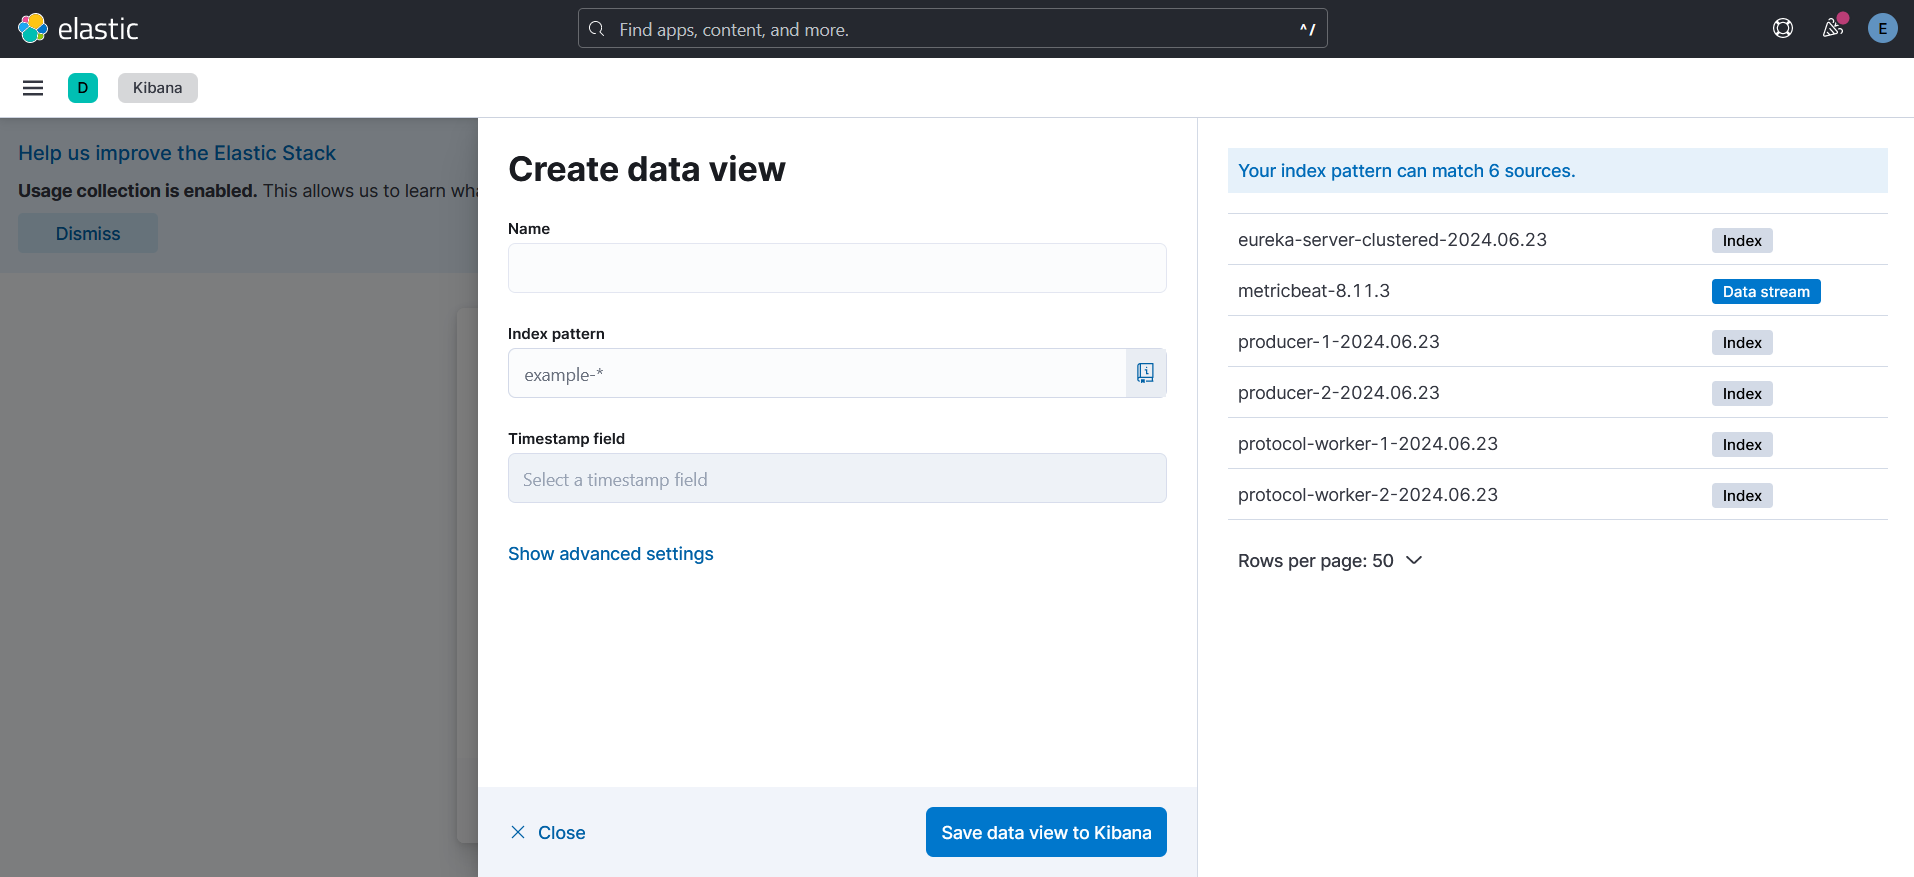
\includegraphics[width=\textwidth]{images/implementation/kibanaDiscoveryDataView.png}
    \caption{Kibana --- przechwycone dzienniki zdarzeń}
    \label{kibanaDiscoveryDataView}
\end{figure}

\subsection{Monitorowanie podsystemu}

Blok "Monitorowanie podsystemu" odbywa się za pośrednictwem usługi Metricbeat, która zbiera i wysyła metryki z różnych systemów i usług. Metricbeat gromadzi metryki na poziomie systemu, takie jak użycie procesora, użycie pamięci, dysku i ruchu sieciowego, następnie wysyła te dane do Elasticsearch. Dane te są następnie analizowane i wizualizowane w usłudze Kibana, zapewniając kompleksowe monitorowanie wydajności infrastruktury, kondycji i wykorzystania zasobów.

\section{Uruchomienie środowiska}

\subsection{Bazowe środowisko}

W celu uruchomienia systemu, na komputerze wymagane są zainstalowane narzędzia \verb|Docker| i \verb|Docker Compose|. Głównym plikiem niezbędnym to uruchomienia systemu jest plik \verb|docker-compose.yml| zaprezentowany na listing \ref{dockerComposeFile}, w którym zdefiniowane są usługi monitoringu systemu oraz rozproszony rejestr usług.

\begin{lstlisting}[caption=Plik docker-comose.yml, label=dockerComposeFile]
    version: '3.8'
    
    x-common-elastisearch-image: &elasticsearchImage
      image: docker.elastic.co/elasticsearch/elasticsearch:${STACK_VERSION}
    x-common-logstash-image: &logstashImage
      image: docker.elastic.co/logstash/logstash:${STACK_VERSION}
    x-common-my-eureka-image: &myEureka
      build: Service-registry
      image: my-eureka-builder-image
    
    volumes:
      certs:
        driver: local
      esdata01:
        driver: local
      esdata02:
        driver: local
      esdata03:
        driver: local
      kibanadata:
        driver: local
      metricbeatdata01:
        driver: local
      logstashdata01:
        driver: local
      logstashdata02:
        driver: local
      logstashdata03:
        driver: local
    
    networks:
      masterNetwork:
        driver: bridge
        name: masterNetwork
        ipam:
          config:
            - subnet: 172.20.0.0/16
    
    services:  
      setup:
        container_name: setup
        <<: *elasticsearchImage
        volumes:
          - certs:/usr/share/elasticsearch/config/certs
        user: "0"
        networks:
          masterNetwork:
            ipv4_address: 172.20.0.5
        command: >
          bash -c '
            if [ x${ELASTIC_PASSWORD} == x ]; then
              echo "Set the ELASTIC_PASSWORD environment variable in the .env file";
              exit 1;
            elif [ x${KIBANA_PASSWORD} == x ]; then
              echo "Set the KIBANA_PASSWORD environment variable in the .env file";
              exit 1;
            fi;
            if [ ! -f config/certs/ca.zip ]; then
              echo "Creating CA";
              bin/elasticsearch-certutil ca --silent --pem -out config/certs/ca.zip;
              unzip config/certs/ca.zip -d config/certs;
            fi;
            if [ ! -f config/certs/certs.zip ]; then
              echo "Creating certs";
              echo -ne \
              "instances:\n"\
              "  - name: es01\n"\
              "    dns:\n"\
              "      - es01\n"\
              "      - localhost\n"\
              "    ip:\n"\
              "      - 127.0.0.1\n"\
              "  - name: es02\n"\
              "    dns:\n"\
              "      - es02\n"\
              "      - localhost\n"\
              "    ip:\n"\
              "      - 127.0.0.1\n"\
              "  - name: es03\n"\
              "    dns:\n"\
              "      - es03\n"\
              "      - localhost\n"\
              "    ip:\n"\
              "      - 127.0.0.1\n"\
              "  - name: kibana\n"\
              "    dns:\n"\
              "      - kibana\n"\
              "      - localhost\n"\
              "    ip:\n"\
              "      - 127.0.0.1\n"\
              > config/certs/instances.yml;
              bin/elasticsearch-certutil cert --silent --pem -out config/certs/certs.zip --in config/certs/instances.yml --ca-cert config/certs/ca/ca.crt --ca-key config/certs/ca/ca.key;
              unzip config/certs/certs.zip -d config/certs;
            fi;
            echo "Setting file permissions"
            chown -R root:root config/certs;
            find . -type d -exec chmod 750 \{\} \;;
            find . -type f -exec chmod 640 \{\} \;;
            echo "Waiting for Elasticsearch availability";
            until curl -s --cacert config/certs/ca/ca.crt https://es01:9200 | grep -q "missing authentication credentials"; do sleep 30; done;
            echo "Setting kibana_system password";
            until curl -s -X POST --cacert config/certs/ca/ca.crt -u "elastic:${ELASTIC_PASSWORD}" -H "Content-Type: application/json" https://es01:9200/_security/user/kibana_system/_password -d "{\"password\":\"${KIBANA_PASSWORD}\"}" | grep -q "^{}"; do sleep 10; done;
            echo "All done!";
          '
        healthcheck:
          test: ["CMD-SHELL", "[ -f config/certs/es01/es01.crt ]"]
          interval: 1s
          timeout: 5s
          retries: 120
    
      es01:
        container_name: elasticsearch01
        depends_on:
          setup:
            condition: service_healthy
        <<: *elasticsearchImage
        volumes:
          - certs:/usr/share/elasticsearch/config/certs
          - esdata01:/usr/share/elasticsearch/data
        ports:
          - ${ES_PORT}:9200
        networks:
          masterNetwork:
            ipv4_address: 172.20.0.6
        environment:
          - node.name=es01
          - cluster.name=${CLUSTER_NAME}
          - cluster.initial_master_nodes=es01,es02,es03
          - discovery.seed_hosts=es02,es03
          - ELASTIC_PASSWORD=${ELASTIC_PASSWORD}
          - bootstrap.memory_lock=true
          - xpack.security.enabled=true
          - xpack.security.http.ssl.enabled=true
          - xpack.security.http.ssl.key=certs/es01/es01.key
          - xpack.security.http.ssl.certificate=certs/es01/es01.crt
          - xpack.security.http.ssl.certificate_authorities=certs/ca/ca.crt
          - xpack.security.transport.ssl.enabled=true
          - xpack.security.transport.ssl.key=certs/es01/es01.key
          - xpack.security.transport.ssl.certificate=certs/es01/es01.crt
          - xpack.security.transport.ssl.certificate_authorities=certs/ca/ca.crt
          - xpack.security.transport.ssl.verification_mode=certificate
          - xpack.license.self_generated.type=${LICENSE}
          - xpack.monitoring.collection.enabled=true
        mem_limit: 1g
        deploy:
          resources:
            limits:
              cpus: '0.5'
              memory: 1g
        ulimits:
          memlock:
            soft: -1
            hard: -1
        healthcheck:
          test:
            [
              "CMD-SHELL",
              "curl -s --cacert config/certs/ca/ca.crt https://localhost:9200 | grep -q 'missing authentication credentials'",
            ]
          interval: 10s
          timeout: 10s
          retries: 120
    
      es02:
        container_name: elasticsearch02
        depends_on:
          - es01
        <<: *elasticsearchImage
        networks:
          masterNetwork:
            ipv4_address: 172.20.0.7
        volumes:
          - certs:/usr/share/elasticsearch/config/certs
          - esdata02:/usr/share/elasticsearch/data
        environment:
          - node.name=es02
          - cluster.name=${CLUSTER_NAME}
          - cluster.initial_master_nodes=es01,es02,es03
          - discovery.seed_hosts=es01,es03
          - ELASTIC_PASSWORD=${ELASTIC_PASSWORD}
          - bootstrap.memory_lock=true
          - xpack.security.enabled=true
          - xpack.security.http.ssl.enabled=true
          - xpack.security.http.ssl.key=certs/es02/es02.key
          - xpack.security.http.ssl.certificate=certs/es02/es02.crt
          - xpack.security.http.ssl.certificate_authorities=certs/ca/ca.crt
          - xpack.security.transport.ssl.enabled=true
          - xpack.security.transport.ssl.key=certs/es02/es02.key
          - xpack.security.transport.ssl.certificate=certs/es02/es02.crt
          - xpack.security.transport.ssl.certificate_authorities=certs/ca/ca.crt
          - xpack.security.transport.ssl.verification_mode=certificate
          - xpack.license.self_generated.type=${LICENSE}
          - xpack.monitoring.collection.enabled=true
        mem_limit: 1g
        deploy:
          resources:
            limits:
              cpus: '0.5'
              memory: 1g
        ulimits:
          memlock:
            soft: -1
            hard: -1
        healthcheck:
          test:
            [
              "CMD-SHELL",
              "curl -s --cacert config/certs/ca/ca.crt https://localhost:9200 | grep -q 'missing authentication credentials'",
            ]
          interval: 10s
          timeout: 10s
          retries: 120
    
      es03:
        container_name: elasticsearch03
        depends_on:
          - es02
        <<: *elasticsearchImage
        networks:
          masterNetwork:
            ipv4_address: 172.20.0.8
        volumes:
          - certs:/usr/share/elasticsearch/config/certs
          - esdata03:/usr/share/elasticsearch/data
        environment:
          - node.name=es03
          - cluster.name=${CLUSTER_NAME}
          - cluster.initial_master_nodes=es01,es02,es03
          - discovery.seed_hosts=es01,es02
          - ELASTIC_PASSWORD=${ELASTIC_PASSWORD}
          - bootstrap.memory_lock=true
          - xpack.security.enabled=true
          - xpack.security.http.ssl.enabled=true
          - xpack.security.http.ssl.key=certs/es03/es03.key
          - xpack.security.http.ssl.certificate=certs/es03/es03.crt
          - xpack.security.http.ssl.certificate_authorities=certs/ca/ca.crt
          - xpack.security.transport.ssl.enabled=true
          - xpack.security.transport.ssl.key=certs/es03/es03.key
          - xpack.security.transport.ssl.certificate=certs/es03/es03.crt
          - xpack.security.transport.ssl.certificate_authorities=certs/ca/ca.crt
          - xpack.security.transport.ssl.verification_mode=certificate
          - xpack.license.self_generated.type=${LICENSE}
          - xpack.monitoring.collection.enabled=true
        mem_limit: 1g
        deploy:
          resources:
            limits:
              cpus: '0.5'
              memory: 1g
        ulimits:
          memlock:
            soft: -1
            hard: -1
        healthcheck:
          test:
            [
              "CMD-SHELL",
              "curl -s --cacert config/certs/ca/ca.crt https://localhost:9200 | grep -q 'missing authentication credentials'",
            ]
          interval: 10s
          timeout: 10s
          retries: 120
    
      kibana:
        container_name: kibana
        depends_on:
          es01:
            condition: service_healthy
          es02:
            condition: service_healthy
          es03:
            condition: service_healthy
        image: docker.elastic.co/kibana/kibana:${STACK_VERSION}
        volumes:
          - certs:/usr/share/kibana/config/certs
          - kibanadata:/usr/share/kibana/data
        ports:
          - ${KIBANA_PORT}:5601
        networks:
          masterNetwork:
            ipv4_address: 172.20.0.9
        environment:
          - SERVERNAME=kibana
          - ELASTICSEARCH_HOSTS=["https://es01:9200","https://es02:9200","https://es03:9200"]
          - ELASTICSEARCH_USERNAME=kibana_system
          - ELASTICSEARCH_PASSWORD=${KIBANA_PASSWORD}
          - ELASTICSEARCH_SSL_CERTIFICATEAUTHORITIES=config/certs/ca/ca.crt
          - XPACK_SECURITY_ENCRYPTIONKEY=${ENCRYPTION_KEY}
          - XPACK_ENCRYPTEDSAVEDOBJECTS_ENCRYPTIONKEY=${ENCRYPTION_KEY}
          - XPACK_REPORTING_ENCRYPTIONKEY=${ENCRYPTION_KEY}
        mem_limit: 1g
        deploy:
          resources:
            limits:
              cpus: '0.5'
              memory: 1g
        healthcheck:
          test:
            [
              "CMD-SHELL",
              "curl -s -I http://localhost:5601 | grep -q 'HTTP/1.1 302 Found'",
            ]
          interval: 10s
          timeout: 10s
          retries: 120
    
      logstash01:
        <<: *logstashImage
        container_name: logstash01
        ports:
          - 5000:5000
        depends_on:
          es01:
            condition: service_healthy
          es02:
            condition: service_healthy
          es03:
            condition: service_healthy
          kibana:
            condition: service_healthy
        labels:
          co.elastic.logs/module: logstash
        user: root
        networks:
          masterNetwork:
            ipv4_address: 172.20.0.12
        volumes:
          - certs:/usr/share/logstash/certs
          - logstashdata01:/usr/share/logstash/data
          - "./ELK-monitoring/logstash_ingest_data/:/usr/share/logstash/ingest_data/"
          - "./ELK-monitoring/logstashConfig/pipeline:/usr/share/logstash/pipeline:ro"
        environment:
          - xpack.monitoring.enabled=true
          - xpack.monitoring.collection.enabled=true
          - xpack.monitoring.elasticsearch.hosts=["https://es01:9200","https://es02:9200","https://es03:9200"]
          - xpack.monitoring.elasticsearch.username="elastic"
          - xpack.monitoring.elasticsearch.password=${ELASTIC_PASSWORD}
          - xpack.monitoring.elasticsearch.ssl.certificate_authority=certs/ca/ca.crt
          - ELASTIC_USER=elastic
          - ELASTIC_PASSWORD=${ELASTIC_PASSWORD}
        mem_limit: 512m
        deploy:
          resources:
            limits:
              cpus: '0.25'
              memory: 512m
        healthcheck:
          test: [
            "CMD-SHELL",
            "curl -XGET 'localhost:9600/_node/stats'"
          ]
          interval: 30s
          timeout: 10s
          retries: 120
    
      logstash02:
        <<: *logstashImage
        container_name: logstash02
        ports:
          - 5001:5000
        depends_on:
          es01:
            condition: service_healthy
          es02:
            condition: service_healthy
          es03:
            condition: service_healthy
          kibana:
            condition: service_healthy
        labels:
          co.elastic.logs/module: logstash
        user: root
        networks:
          masterNetwork:
            ipv4_address: 172.20.0.13
        volumes:
          - certs:/usr/share/logstash/certs
          - logstashdata02:/usr/share/logstash/data
          - "./ELK-monitoring/logstash_ingest_data/:/usr/share/logstash/ingest_data/"
          - "./ELK-monitoring/logstashConfig/pipeline:/usr/share/logstash/pipeline:ro"
        environment:
          - xpack.monitoring.enabled=true
          - xpack.monitoring.collection.enabled=true
          - xpack.monitoring.elasticsearch.hosts=["https://es01:9200","https://es02:9200","https://es03:9200"]
          - xpack.monitoring.elasticsearch.username="elastic"
          - xpack.monitoring.elasticsearch.password=${ELASTIC_PASSWORD}
          - xpack.monitoring.elasticsearch.ssl.certificate_authority=certs/ca/ca.crt
          - ELASTIC_USER=elastic
          - ELASTIC_PASSWORD=${ELASTIC_PASSWORD}
        mem_limit: 512m
        deploy:
          resources:
            limits:
              cpus: '0.25'
              memory: 512m
        healthcheck:
          test: [
            "CMD-SHELL",
            "curl -XGET 'localhost:9600/_node/stats'"
          ]
          interval: 30s
          timeout: 10s
          retries: 120
    
      logstash03:
        <<: *logstashImage
        container_name: logstash03
        ports:
          - 5002:5000
        depends_on:
          es01:
            condition: service_healthy
          es02:
            condition: service_healthy
          es03:
            condition: service_healthy
          kibana:
            condition: service_healthy
        labels:
          co.elastic.logs/module: logstash
        user: root
        networks:
          masterNetwork:
            ipv4_address: 172.20.0.14
        volumes:
          - certs:/usr/share/logstash/certs
          - logstashdata03:/usr/share/logstash/data
          - "./ELK-monitoring/logstash_ingest_data/:/usr/share/logstash/ingest_data/"
          - "./ELK-monitoring/logstashConfig/pipeline:/usr/share/logstash/pipeline:ro"
        environment:
          - xpack.monitoring.enabled=true
          - xpack.monitoring.collection.enabled=true
          - xpack.monitoring.elasticsearch.hosts=["https://es01:9200","https://es02:9200","https://es03:9200"]
          - xpack.monitoring.elasticsearch.username="elastic"
          - xpack.monitoring.elasticsearch.password=${ELASTIC_PASSWORD}
          - xpack.monitoring.elasticsearch.ssl.certificate_authority=certs/ca/ca.crt
          - ELASTIC_USER=elastic
          - ELASTIC_PASSWORD=${ELASTIC_PASSWORD}
        mem_limit: 512m
        deploy:
          resources:
            limits:
              cpus: '0.25'
              memory: 512m
        healthcheck:
          test: [
            "CMD-SHELL",
            "curl -XGET 'localhost:9600/_node/stats'"
          ]
          interval: 30s
          timeout: 10s
          retries: 120
    
      metricbeat01:
        container_name: metricbeat01
        depends_on:
          es01:
            condition: service_healthy
          es02:
            condition: service_healthy
          es03:
            condition: service_healthy
          kibana:
            condition: service_healthy
        image: docker.elastic.co/beats/metricbeat:${STACK_VERSION}
        user: root
        networks:
          masterNetwork:
            ipv4_address: 172.20.0.10
        volumes:
          - certs:/usr/share/metricbeat/certs
          - metricbeatdata01:/usr/share/metricbeat/data
          - "./ELK-monitoring/metricbeat.yml:/usr/share/metricbeat/metricbeat.yml:ro"
          - "/var/run/docker.sock:/var/run/docker.sock:ro"
          - "/sys/fs/cgroup:/hostfs/sys/fs/cgroup:ro"
          - "/proc:/hostfs/proc:ro"
          - "/:/hostfs:ro"
        environment:
          - ELASTIC_USER=elastic
          - ELASTIC_PASSWORD=${ELASTIC_PASSWORD}
          - ELASTIC_HOSTS=["https://es01:9200","https://es02:9200","https://es03:9200"]
          - KIBANA_HOSTS=http://kibana:5601
          - LOGSTASH_HOSTS=["http://logstash01:9600","http://logstash02:9600","http://logstash03:9600"]
        mem_limit: 512m
        deploy:
          resources:
            limits:
              cpus: '0.25'
              memory: 512m
    
      eureka-server-peer-1:
        <<: *myEureka
        depends_on:
          logstash01:
            condition: service_healthy
          logstash02:
            condition: service_healthy
          logstash03:
            condition: service_healthy
        container_name: eureka-server-peer-1
        ports:
          - "9001:9001"
        environment:
          - SPRING_PROFILES_ACTIVE=peer-1
          - PEER_2_URL=http://172.20.0.3:9002/eureka/
          - PEER_3_URL=http://172.20.0.4:9003/eureka/
          - LOGSTASH_DESTINATION_ONE=172.20.0.12:5000
          - LOGSTASH_DESTINATION_TWO=172.20.0.13:5000
          - LOGSTASH_DESTINATION_THREE=172.20.0.14:5000
        networks:
          masterNetwork:
            ipv4_address: 172.20.0.2
        mem_limit: 1g
        deploy:
          resources:
            limits:
              cpus: '0.5'
              memory: 1g
    
      eureka-server-peer-2:
        <<: *myEureka
        depends_on:
          logstash01:
            condition: service_healthy
          logstash02:
            condition: service_healthy
          logstash03:
            condition: service_healthy
        container_name: eureka-server-peer-2
        ports:
          - "9002:9002"
        environment:
          - SPRING_PROFILES_ACTIVE=peer-2
          - PEER_1_URL=http://172.20.0.2:9001/eureka/
          - PEER_3_URL=http://172.20.0.4:9003/eureka/
          - LOGSTASH_DESTINATION_ONE=172.20.0.12:5000
          - LOGSTASH_DESTINATION_TWO=172.20.0.13:5000
          - LOGSTASH_DESTINATION_THREE=172.20.0.14:5000
        networks:
          masterNetwork:
            ipv4_address: 172.20.0.3
        mem_limit: 1g
        deploy:
          resources:
            limits:
              cpus: '0.5'
              memory: 1g
    
      eureka-server-peer-3:
        <<: *myEureka
        depends_on:
          logstash01:
            condition: service_healthy
          logstash02:
            condition: service_healthy
          logstash03:
            condition: service_healthy
        container_name: eureka-server-peer-3
        ports:
          - "9003:9003"
        environment:
          - SPRING_PROFILES_ACTIVE=peer-3
          - PEER_1_URL=http://172.20.0.2:9001/eureka/
          - PEER_2_URL=http://172.20.0.3:9002/eureka/
          - LOGSTASH_DESTINATION_ONE=172.20.0.12:5000
          - LOGSTASH_DESTINATION_TWO=172.20.0.13:5000
          - LOGSTASH_DESTINATION_THREE=172.20.0.14:5000
        networks:
          masterNetwork:
            ipv4_address: 172.20.0.4
        mem_limit: 1g
        deploy:
          resources:
            limits:
              cpus: '0.5'
              memory: 1g
\end{lstlisting}

Bloki x--common--elastisearch--image, x-common--logstash--image i x--common--my--eureka--image definiują informacje o konfiguracji wielokrotnego użytku odpowiednio dla Elasticsearch, Logstash i obrazu rejestru usług. Są one wykorzystywane w celu uniknięcia powtórzeń definicji obrazu w poszczególnych usługach.

Sekcja woluminów definiuje trwałe obszary przechowywania dla poszczególnych kontenerów.

Sekcja sieci, definiuje sieć razem z podsiecią łączącą usługi w ramach uruchamianego środowiska.

Podstawowe środowisko składa się z następujących usług:
\begin{itemize}
    \item Usługa \verb|setu| inicjuje certyfikaty Elasticsearch. 
    \item Zdefiniowane są trzy węzły Elasticsearch (es01, es02, es03). Są one zależne od usługi \verb|setup|. Każda z tych usług przyjmuje w polu \verb|discovery.seed_hosts| adresy pozostałych uruchomionych usług Elasticsearch w celu utworzenia klastra usług zapewniającego wysoką dostępność.
    \item Usługa \verb|Kibana| łączy się z klastrem Elasticsearch w celu dostępu do zbieranych dokumentów i wizualizacji danych w interfejsie sieciowym uruchomionym na porcie 5601.
    \item Trzy instancje Logstash (logstash01, logstash02, logstash03) są zdefiniowane do obsługi pozyskiwania i przetwarzania danych. Każda instancja Logstash przyjmuje jako argument każdy węzeł z uruchomionego klastra Elasticsearch w celu zapewnienia wysokiej dostępności w razie awarii węzłów w klastrze.
    \item Usługa metricbeat01 służy do zbierania metryk z innych usług ze stosu ELK i wysyłania tych metryk do Elasticsearch.
    \item Trzy instancje serwera Eureka (eureka--server--peer--1, eureka--server--peer--2, eureka--server--peer--3) są zdefiniowane do wykrywania usług. Do każdej usługi są podane zmienne środowiskowo uruchamiające usługę jako wcześniej zdefiniowany profil aplikacyjny w celu uruchomienia klastra rejestrów Eureka.
\end{itemize}

Aby uruchomić powyższą konfigurację Docker Compose, należy użyć następującego polecenia:

\begin{verbatim}
sudo docker compose --env-file ELK-monitoring/.env down -v && \
sudo docker compose --env-file ELK-monitoring/.env build --no-cache && \
sudo docker compose --env-file ELK-monitoring/.env up --force-recreate -d
\end{verbatim}

Powyższe polecenie wykonuje następujące czynności:

\begin{itemize}
    \item Zatrzymuje i usuwa wszystkie uruchomione usługi i woluminy.
    \item Buduje obrazy Docker bez użycia pamięci podręcznej.
    \item Uruchamia usługi, wymuszając odtworzenie kontenerów i uruchomienie ich w trybie odłączonym.
\end{itemize}

Opisany powyżej plik \verb|docker-compose.yml| konfiguruje środowisko rozruchowe klastra Elasticsearch, wraz z instancjami Logstash do przetwarzania danych, Kibana do wizualizacji, Metricbeat do zbierania metryk i konfiguracją serwera Eureka do wykrywania usług w systemie. Usługi są połączone za pomocą sieci Docker, a trwałe przechowywanie w przypadku wyłączenia systemu jest zarządzane za pomocą woluminów Docker. Wykorzystanie zmiennych środowiskowych i kontroli kondycji zapewnia, że usługi są poprawnie skonfigurowane i uruchamiane w ściśle określonej kolejności.

\subsection{Producent}

Skrypt Bash przedstawiony na listingu\ref{producerBashScript} jest przeznaczony do uruchamiania wielu instancji usługi kontenerowej Docker, z których każda reprezentuje producenta. Skrypt zapewnia dostępność obrazu Docker dla producentów, buduje go w razie potrzeby, a następnie uruchamia określoną liczbę instancji producentów z odpowiednimi zmiennymi środowiskowymi i konfiguracjami sieciowymi.

\begin{lstlisting}[language=bash,caption=Kod skryptu producers.sh,label=producerBashScript]
    #!/bin/bash

    # Check if the necessary arguments are provided
    if [ $# -ne 2 ]; then
        echo "Usage: $0 <first producer id> <number of producers>"
        exit 1
    fi
    
    # First producer ID and number of producers to run
    first_producer_id=$1
    num_producers=$2
    
    # Function to check if the Docker image exists and build it if not
    ensure_docker_image() {
        if [ -z "$(docker images -q producer:latest 2> /dev/null)" ]; then
            echo "'producer:latest' image not found. Building image..."
            if ! docker build Producer -t producer:latest --no-cache; then
                echo "Error building Docker image 'producer:latest'. Exiting."
                exit 1
            fi
        fi
    }
    
    # Ensure the Docker image is available
    ensure_docker_image
    
    # Loop and run the Docker command
    for (( i=first_producer_id; i<first_producer_id+num_producers; i++ )); do
    
        docker run --rm -d --network=masterNetwork \
        -e PEER_1_URL=http://172.20.0.2:9001/eureka/,http://172.20.0.3:9002/eureka/,http://172.20.0.4:9003/eureka/ \
        -e PRODUCER_ID=$i \
        -e LOGSTASH_DESTINATION_ONE=172.20.0.12:5000 \
        -e LOGSTASH_DESTINATION_TWO=172.20.0.13:5000 \
        -e LOGSTASH_DESTINATION_THREE=172.20.0.14:5000 \
        -e NUMBER_OF_PRODUCTS=10 \
        -e PORT=10000 \
        -p $((10000+$i)):10000 \
        --name=PRODUCER_$i producer:latest
    
    done

\end{lstlisting}

Skrypt oczekuje dwóch argumentów: identyfikatora pierwszego producenta i liczby instancji producenta do uruchomienia. Jeżeli te argumenty nie zostaną dostarczone, skrypt wyświetli informacje o braku argumentów i zakończy działanie. Następnie ensure\_docker\_image sprawdza, czy obraz Docker o nazwie \verb|producer:latest| istnieje. Jeśli obraz nie istnieje, buduje obraz z katalogu Producer. Jeśli kompilacja nie powiedzie się, skrypt kończy działanie z komunikatem o błędzie. Następnie skrypt wykonuje pętlę od pierwszego identyfikatora producenta do określonej liczby producentów. Dla każdej iteracji uruchamia kontener Docker z niezbędnymi zmiennymi środowiskowymi i konfiguracjami sieciowymi. Każdy kontener ma unikalną nazwę i jest połączony z siecią \verb|masterNetwork|.

Skrypt \verb|producers.sh| automatyzuje wdrażanie wielu instancji producentów. Zapewnia on dostępność wymaganego obrazu Docker, buduje go w razie potrzeby, a następnie uruchamia określoną liczbę producentów z odpowiednimi konfiguracjami. Ta konfiguracja jest przydatna do testowania i skalowania usług producentów w kontrolowanym środowisku.

\subsection{Węzeł protokołu}

Skrypt przedstawiony na listingu\ref{workersBashScript} jest przeznaczony do uruchamiania wielu instancji aplikacji kontenerowej Docker, z których każda reprezentuje węzeł protokołu. Skrypt zapewnia dostępność obrazu Docker dla węzła protokołu, buduje go w razie potrzeby, a następnie uruchamia określoną liczbę instancji węzłów z odpowiednimi zmiennymi środowiskowymi i konfiguracjami sieciowymi.

\begin{lstlisting}[language=bash,caption=Kod skryptu workers.sh,label=workersBashScript]
    #!/bin/bash

    # Check if the necessary arguments are provided
    if [ $# -ne 2 ]; then
        echo "Usage: $0 <first worker id> <number of workers>"
        exit 1
    fi
    
    # First producer ID and number of producers to run
    first_worker_id=$1
    num_workers=$2
    
    # Function to check if the Docker image exists and build it if not
    ensure_docker_image() {
        if [ -z "$(docker images -q worker:latest 2> /dev/null)" ]; then
            echo "'worker:latest' image not found. Building image..."
            if ! docker build Master-Protocol-Worker -t worker:latest --no-cache; then
                echo "Error building Docker image 'worker:latest'. Exiting."
                exit 1
            fi
        fi
    }
    
    # Ensure the Docker image is available
    ensure_docker_image
    
    # Loop and run the Docker command
    for (( i=first_worker_id; i<first_worker_id+num_workers; i++ )); do
    
        docker run --rm -d --network=masterNetwork \
        -e PEER_1_URL=http://172.20.0.2:9001/eureka/,http://172.20.0.3:9002/eureka/,http://172.20.0.4:9003/eureka/ \
        -e WORKER_ID=$i \
        -e LOGSTASH_DESTINATION_ONE=172.20.0.12:5000 \
        -e LOGSTASH_DESTINATION_TWO=172.20.0.13:5000 \
        -e LOGSTASH_DESTINATION_THREE=172.20.0.14:5000 \
        -e PORT=11000\
        -p $((12000+$i)):11000 \
        --name=Worker-$i \
        worker
    
    done
\end{lstlisting}

Skrypt oczekuje dwóch argumentów: identyfikatora pierwszego węzła i liczby instancji węzłów do uruchomienia. Jeżeli te argumenty nie zostaną dostarczone, skrypt wyświetli informacje o braku argumentów i zakończy działanie. Funkcja ensure\_docker\_image sprawdza, czy obraz Docker o nazwie \verb|worker:latest| istnieje. Jeżeli obraz nie istnieje, buduje obraz z katalogu Master--Protocol--Worker. Jeśli kompilacja nie powiedzie się, skrypt kończy działanie z komunikatem o błędzie. Następnie skrypt wykonuje pętlę od pierwszego identyfikatora węzła do określonej liczby węzłów. Dla każdej iteracji uruchamia kontener Docker z niezbędnymi zmiennymi środowiskowymi i konfiguracjami sieciowymi. Każdy kontener ma unikalną nazwę i jest połączony z siecią \verb|masterNetwork|.

Skrypt automatyzuje wdrażanie wielu instancji roboczych w sieci Docker. Zapewnia on dostępność wymaganego obrazu Docker, buduje go w razie potrzeby, a następnie uruchamia określoną liczbę pracowników z odpowiednimi konfiguracjami. Ta konfiguracja jest przydatna do testowania i skalowania usług roboczych w kontrolowanym środowisku.
